%!TEX root = ../../Heun_Dale_Haney_A_dynamic_approach_to_input_output_modeling.tex
%%%%%%%%%%%%%%%%%%%%% chapter.tex %%%%%%%%%%%%%%%%%%%%%%%%%%%%%%%%%
%
% sample chapter
%
% Use this file as a template for your own input.
%
%%%%%%%%%%%%%%%%%%%%%%%% Springer-Verlag %%%%%%%%%%%%%%%%%%%%%%%%%%
%\motto{Use the template \emph{chapter.tex} to style the various elements of your chapter content.}
\motto{Well, I have my rights, sir, 
and I'm telling you I intend to go on doing just what I do! 
And, for your information, you Lorax, 
I'm figgering on biggering and BIGGERING and \large BIGGERING
\small and \Large BIGGERING\small \ldots~\emph{\cite{Seuss:1971aa}}

\hfill---\emph{The Once-ler}}

\chapter{Material flows}
% use \chaptermark{}
% to alter or adjust the chapter heading in the running head
\chaptermark{Materials}
% Always give a unique label
\label{chap:materials} 

\abstract*{In this chapter we will develop a framework 
for accounting material flows and accumulations
within economies.
We will begin by looking at accounting in everyday life
before using concepts from thermodynamics, 
such as system boundaries, control volumes as well as
the First Law of Thermodynamics,
to develop a rigorous accounting procedure.
This procedure is applied first to a one-sector then 
two-sector model of the economy,
in order to build up to a general framework for material
accounting.
We then apply the framework to the real-world
example of the US auto industry.
 }


%% \abstract{Each chapter should be preceded by an abstract (10--15 lines long) that summarizes the content. The abstract will appear \textit{online} at \url{www.SpringerLink.com} and be available with unrestricted access. This allows unregistered users to read the abstract as a teaser for the complete chapter. As a general rule the abstracts will not appear in the printed version of your book unless it is the style of your particular book or that of the series to which your book belongs.\newline\indent
%% Please use the 'starred' version of the new Springer \texttt{abstract} command for typesetting the text of the online abstracts (cf. source file of this chapter template \texttt{abstract}) and include them with the source files of your manuscript. Use the plain \texttt{abstract} command if the abstract is also to appear in the printed version of the book.}

%% Use the template \emph{chapter.tex} together with the Springer document class SVMono (monograph-type books) or SVMult (edited books) to style the various elements of your chapter content in the Springer layout.

In Chapter~\ref{chap:intro}, we put forward the idea that 
the economy is society's metabolism.
This chapter explores
this idea further by observing the interchange of materials \emph{within}
an economy, as well as exchanges of materials between an economy and 
surrounding environment---the biosphere. 

% [THE FOLLOWING PARAGRAPH CONNECTS MORE WITH THE METABOLISM METAPHOR,
% NEED TO DECIDE BETWEEN THAT AND THE ONE AFTER OR MAYBE MIX THE TWO]

% Just as a living organism takes
% in food, water and air, so too an
% economy must take in raw materials from its environment. To a large extent,
% the major exchanges of materials between industrial economies and their 
% environment mirror those of an animal. Large inputs of fresh water, hydrocarbons
% and oxygen with the emission of carbon dioxide and polluted water [REF BRANDT]
% dioxide and hydro-carbons These
% materials are then used for a number of different purposes. Some
% become the building blocks from which the physical structures within the 
% economy---buildings, roads, even people---are composed. These materials
% must be extracted from the environment and processed, transported and then
% manufactured into final goods. Such activities require energy resources. In
% an economy primarily dependent on the combustion of fossil fuels, energy conversion
% of energy necessarily requires the presence of oxygen in the atmosphere and
% the emission of carbon dioxide. Many processes also require flows of materials, 
% especially fresh water, that are not directly embodied in the final product.
 

There are many easily observable instances 
of material accumulations
within an economy. 
A typical office contains a computer screen, coffee cup
and myriad other items. 
Beyond the window, there is a street and building
opposite. 

There are also innumerable material flows caused by an economy 
that most of us do not observe.
The extraction of raw materials generates additional overburden---earth that must be
extracted and processed and ultimately discarded without ever entering the economy
proper. 
Other flows occur around us unseen. 
The cars outside in the street suck in nitrogen and oxygen 
(without which the engine would not work) 
and emit water, carbon dioxide, and
other, more harmful, wastes. 

Even services that we consider ``non-material'' require at least some material
infrastructure. The hairdresser requires scissors (and to a greater or lesser extent 
some hair) with which to work. 
Even the internet, 
often lauded as the exemplar of
dematerialization of the economic process, 
requires a whole host of
infrastructure including 
uninterrupted electricity, 
data servers, 
telephone networks, and 
a computer by which to access it.

It almost goes without saying that 
all materials within the economy (the \emph{econosphere}~\cite{Boulding1966})
started their ``lives'' within the biosphere,
be they food, water or paper, petroleum or rock. 
%They were extracted and processed, transported and
%transformed requiring yet more materials and energy inputs in the form of
%electricity or fuels.
In fact,
the economy is in a continual state of material exchange
with the surrounding environment;
raw materials are pulled in wastes are emitted.
It is this exchange that intimately couples the two spheres,
intertwining their mutual fate.

As discussed in the Preface,
researchers are beginning to quantify these material exchanges.
Further work, such as that by 
the United Nations Environment Programme (UNEP)
International Resource Panel (IRP),
is attempting to measure 
the total stock of materials within society.\cite{Graedel2010}
Over the past two centuries,
human demand for materials has increased at a phenomenal pace.
This demand has driven ever increasing extraction of raw materials 
from the biosphere.
Production of all materials increased from
around 12 Gt (10$^9$~t) to 
around 35 Gt in the period 1945-1980 and up to
68 Gt by the year 2009.\cite{Krausmann2009}
That is, the flow of materials 
into the economy from the biosphere
has grown over five-fold
since the end of the Second World War
and has doubled in the last thirty years.
But what has driven this incredible growth?

An obvious answer to this question is population.
The global population has increased by a factor of 
nearly three during the post-war period.\cite{UNPD2013}
More people obviously leads to greater demand.
Living standards have also increased,
leading to still greater demands for material possessions.
The UNEP-IRP report,
\emph{Metal Stocks in Society} estimates that
if the global in-use per capita stock of metals were to
increase to the level of industrialized nations,
the total stock might be 3-9 times the present level.\cite{Graedel2010}

**** MCD - try to reduce treadmill logic to fewer bullet points ****
**** MCD - done this. Becky, does the footnote look better now? ****

A less obvious answer comes from social science.
In 1980, Schnaiberg~\cite{schnaiberg1980} introduced the concept of 
the ``treadmill of production'' to describe the systemic process of
ever-increasing capital investment (and thus demand for materials)
inherent in capitalist society.\footnote{
	The logic of the treadmill is:
 		\begin{enumerate}[noitemsep,topsep=0pt]
 			\item 	capital (production equipment)
 						is accumulating in Western economies, 
 						to replace production labor 
 						with technologies to increase profits; 
 			\item 	these technologies require far more materials and/or energy 
 						to replace previous, labor-intensive processes;
% 			\item 	new technologies emerge from the organization of scientific and 
% 						technological research in universities and research institutes, 
% 						as well as in the new ``research and development'' departments of large firms;
 			\item 	moreover, unlike the prior use of labor, 
 						the new technologies represent forms of sunk capital;
 			\item 	because worker inputs can more readily be cut back 
 						(as opposed to fixed costs of machine operations for sunk capital)
 						labor is further reduced to sustain production at higher levels;
 			\item	yet more capital is added to replace further reduced levels
 						of labor.~\cite[p.296]{Gould2004}
		 \end{enumerate}
 }
% \begin{quote}
% 	Each round of investment weakened the employment situation 
% 	for production workers and worsened environmental conditions, 
% 	but it increased profits. 
% 	For workers, this treadmill implied that increasing investment 
% 	was needed to employ each production worker. 
% 	For ecosystems, each level of resource extraction became 
% 	commodified into new profits and new investments, 
% 	which led to still more rapid increases in demand 
% 	for ecosystem elements.~\cite[p.296]{Gould2004}
% \end{quote}
The treadmill leads to ``higher and higher levels of demand for natural resources 
for a given level of social welfare''.\cite[p.297]{Gould2004}
The treadmill of production is evident today, 
driving up demand for many commodities.
From an economic stand-point we may view the treadmill
as the strive for productivity in factors of production.
In the substitution of capital for labor,
total factor productivity is increased.
The substitution increases the requirement for natural resources
(particularly energy to drive the capital equipment),
but these are assumed to be ``free'' within economic models,
hence do not count towards productivity;
the substitution gets a free productivity boost from nature.

But what about the downstream effects of this increased materials extraction?
Obviously all of that ``stuff'' has to go somewhere.
As our economies pull in more materials from the biosphere,
so too do they expel more wastes,
leading to an increase in total throughput of materials.
As we pointed out at the start of this chapter,
not all materials flow straight through the economy.
They accumulative as objects: buildings, cars, and even people.

%Because economic activity requires energy, 
%we need to understand the way energy flows through economies. 
%The steady-state I-O techniques of Bullard, Herendeen, 
%and others~\cite{Bullard1975,Herendeen1978} 
%offer a means to that end. 
%We contend, however, that these techniques 
%need to be extended and modified 
%to include transient effects 
%that arise when durability of goods and infrastructure 
%(and associated embodied energy) are considered. 

When accumulation is not accounted for,
the assumption is that all flows in and out balance
instantaneously.
Imagine a bath tub where the water flowing in
through the tap is exactly balanced by the water
flowing out the plughole.
The state of the system 
(the amount of water within the bath) is 
fixed---therefore we say the system is in
steady-state.
Or, imagine a growing baby.
The inputs of food and other materials,
though small compared to an adult,
exceed the output of excreta
(gas, solid, and liquid).
While this may be hard for new parents to believe
(how can there be possibly be more going in than is coming out!),
it is simply this imbalance that induces the growth of the baby.
Materials accumulate within the baby's body.
Obviously, 
this imbalance (and the subsequent growth induced)
slows as the child grows up to adulthood.
Nevertheless,
adults still maintain the ability to accumulate
materials.
We can gain (or lose) weight;
a fact to which any yo-yo dieter will readily attest.

Both population and capital equipment are stocks;
accumulations that have built up over time.
We contend that stocks are the drivers of demand,
of flows of materials.
People demand food, clothing, shelter, all of the basic necessities of life,
as well as all of the trappings of modern life; buildings, vehicles, and computers.
The delivery of all of these material wants requires
capital equipment;
more stocks which also have needs.
They require flows of materials and energy to build, operate and maintain them.
This is why we assert that,
in order to properly understand the economic structure
and the real drivers of change,
we must understand the accumulation of materials within our economies.

In the rest of this chapter, we will define a mathematical accounting framework 
to track the flow and accumulation of
materials within an economy, 
building from a one-sector economy up to examples of both
two- and three-sector economies. 
We will finally apply this framework to the illustrative
example of the US automobile industry that runs through the whole book. 
First, we outline the basic methodology.

\section{Methodology}
\label{sec:Materials_Methodology}

% Everyone is familiar with the notion of accounting of material (and even non-material)
% things. In order to be rigorous, the first step requires the definition of what we
% will be counting as well as the place (defined in both time and space) for which we will
% be counting. Engineers often call this a \emph{control volume}. For example, I may wish
% to account the number of apples in my home over a week-long period. In which case,
% I would count the number of apples that enter  and leave my home, as well as any apples
% that are eaten and, just in case I happen to have an apple tree, any apples that grow
% inside my home. Our accounting equation would look something like:

% **** The idea that we are ``counting money'' does not seem exactly 
% right to me. Isn't it that we are accounting for value and energy flows? 
% Later on we will use currency flows to approximate the value flows? BRH ****

This book is about tracking (accounting) flows through the 
economy with a focus on counting materials, energy, and value.
That an entire academic discipline and industry are focused on counting money (``accounting'')
is evidence of its importance in today's economies.
That energy is required to do \emph{anything} is evidence 
of its importance in the economic activity of our daily lives.
And, we believe that the interplay between money and energy
has shaped the past and will continue to influence the future.
In this section, we define rigorous ``counting'' methods that will be applied
to materials, energy and money throughout this book.

%**** Include somewhere in here the difference between \emph{flows} and \emph{funds}, 
%between \emph{efficient cause} and \emph{material cause}. Resources are 
%\emph{transformed} into products.****

\subsection{Accounting in everyday life}
\label{sec:accounting_in_everyday_life}

We all count material (and non-material) stocks and flows every day,
be it the people in a room, the gasoline we consume on our way to work,
or the money in our bank account.
Rigorous counting at the scale of whole economies 
requires precise definition of
\emph{what} we will be counting,
as well as both \emph{when} and \emph{where} 
we will be doing the counting. 
Engineers often call the spatial definition a ``control volume.'' 
Another way to think of creating a
control volume is drawing a boundary. 
What gets counted is what passes through the boundary.
For example, 
we may wish to count (or ``make an accounting of'') 
the stock of apples in our home over the course of a week. 
We draw a spatial boundary (control volume) around our house 
and a temporal boundary ``around'' the week.
We count the apples that enter and leave our home, any
apples that are eaten~(consumed),
and, if we own an apple tree (lucky us!), 
apples that are grown~(produced) during a week. 
A rigorous apple accounting equation, in units of apples, is:
\begin{equation}
	\mathrm{\Delta}\mathrm{apples} 
	= \mathrm{apples~in} 
	- \mathrm{apples~out} 
	+ \mathrm{apples~grown} 
	- \mathrm{apples~eaten}.
\end{equation}

\noindent{}More generally, we may say:
\begin{equation}
	\mathrm{accumulation}
	= \mathrm{transfers~in} 
	- \mathrm{transfers~out}
	+ \mathrm{production}
	- \mathrm{consumption}.
\end{equation}

Notice that, when discussing apples we use the specific terms 
``grown'' and ``eaten,'' 
instead of the more general terms 
``produced'' and ``consumed.''
Later, in Chapter~\ref{chap:value}, when discussing economic value, 
we will use the terms
``generated'' or ``added'' and ``destroyed.'' 
For our purposes, these terms all have equivalent
meanings and we use them interchangeably.

After accounting for the stock of apples in a week,
we can reframe the question to ask,
``at what rate does the stock of apples change 
$\left( \frac{\mathrm{d}a}{\mathrm{d}t} \right)$?'' 
That is, we can examine the rate of
change of the apple stock per unit of time 
relative to the flow of apples ($\dot{a}$), 
in which case our accounting equation becomes:

\begin{equation} \label{eq:apple_rate_accounting}
	\frac{\mathrm{d}a}{\mathrm{d}t}
	= \dot{a}_{in}
	- \dot{a}_{out}
	+ \dot{a}_{grown}
	- \dot{a}_{eaten}
\end{equation}

\noindent{}where the dot above the variable ($\dot{a}$) indicates 
a flow rate per unit time [apples/time] and
the time derivative $\left( \frac{\mathrm{d}a}{\mathrm{d}t} \right)$ 
is the rate of change of the stock of apples per time unit, or more simply,
the accumulation rate.
 
% ***** Take a moment to tie apples to mass or material. 
% Clearly note that material is measured kg rather than dollars.
% Note the distinction between material and mass.
% We are doing material accounting in units of mass.
% We will later do material accounting in units of energy.
% Even later, we will do material accouting in units of dollars. ****

Instead of focusing on apples as our unit of accounting, 
we could track the mass flow 
(in units of mass per unit time,
for instance  [kg/sec]) 
of the main chemical elements within the apples. 
From this perspective, 
although an \emph{apple} may be consumed,
the \emph{elements} of which the apple is 
composed---hydrogen, oxygen (coupled together as water
to form the overwhelming majority of the mass), 
and carbon (which, bonded with hydrogen as carbohydrates make up most 
of the remaining mass)---are \emph{not} consumed. 
They flow through the consumption process unaffected.
The chemical elements will instead be either stored within our body, 
leave the house as waste (in the apple core), 
remain in the house (stored within the apple seed 
that rolled under the sofa)
or, eventually, leave via the air (as carbon dioxide
and water vapor) or otherwise (as excreta) after they have
been metabolized.

%**** Auto industry example here? Perhaps steel? ****

If, instead of a home, we drew a spatial control volume 
around a sector of an economy, 
similar accounting methods can be applied. 
In fact, throughout this book, we will illustrate theoretical concepts with
a running example of a control volume (boundary) around the US auto industry. 
If we account for steel (in units of kg) in the auto industry, 
we might write an equation like this:

\begin{equation}
	\mathrm{\Delta}\mathrm{steel} 
	= \mathrm{steel~in} 
	- \mathrm{steel~out} 
\end{equation}

Note that the production and consumption terms are zero
since steel is not created or destroyed within the automobile
sector. Tracking the rate flows of steel, 
$\dot{s}$ (in kg/s),
we would write the following equation:

\begin{equation}
	\frac{\mathrm{d}s}{\mathrm{d}t}
	= \dot{s}_{in}
	- \dot{s}_{out}
\end{equation}


Again, the last two terms 
(representing steel production and consumption) 
are not present. 
This is in direct contrast with apple 
accounting outlined in Equation~\ref{eq:apple_rate_accounting}. 
%**** Do the previous two sentences make sense?
%The equation has only 2 terms. **** 
%I have reworded to specify the production and consumption terms. ****
Despite the fact that steel is neither produced nor consumed 
within the \emph{automobile sector}, 
there \emph{are} sectors of the economy 
that \emph{do} produce steel,
by mixing molten iron with varying amounts of carbon. 
The flow of steel through an economy illustrates that 
although economic products (steel) 
may be produced or destroyed, 
the mass flows of \emph{elemental materials} 
(iron and other chemical elements)
is unaffected even as the structure changes form (e.g.\ from iron to steel) 
through the many economic processes.\footnote{For the sake of
absolute rigor, we must point out that, in actuality, iron \emph{is} created within
the core of silicon-burning stars. 
Mass and energy may also be converted in such processes, 
such that only mass-energy is conserved. 
However, for the purposes of terrestrial
processes, the total mass (in kg) of iron (Fe) is constant. 
There are, additionally, some economic
processes, within nuclear reactors, that change the atomic structure of elements
and thus violate the accounting law presented here. 
Because the mass flows involved
with these nuclear plants is negligible compared with total materials flows, we
shall assume that the mass of elements are conserved for this book.}
In fact, we may go further.
Every act of economic production
has an associated act of consumption or destruction.
% **** Discuss the steel industry. 
% Show how steel is actually formed from other materials.
% Show that \emph{mass} is neither created nor destroyed, 
% but it may change form. ****
Indeed, within the car industry, inputs of steel, glass, plastic, rubber, etc.\ 
are \emph{consumed} in the very process of producing cars, 
such that \emph{cars} are (literally) \emph{created}
within the automobile industry. 
You can't make an omelet without breaking a few eggs;
you can't make a car without consuming a few sheets of steel.
An accounting equation for cars within the economy
must include terms for production and destruction\footnote{In economic terms,
destruction of physical goods is often called ``depreciation.'' We shall 
explore the importance of and distinctions between 
physical depreciation and economic depreciation 
in Chapters~\ref{chap:embodied_energy}--\ref{chap:implications}.}
of cars.
Again, focusing on mass flows of the chemical elements avoids this necessity, 
because mass is \emph{conserved} in physical processes.
Any mass entering a control volume (transfer in) 
must go somewhere, 
whether it stays within the volume (accumulation) 
or is transferred out.
Conservation of mass is expressed in equations such as the ones above
for apples in a home and steel in the auto industry. 

Another important conservation principle is the conservation of energy.
Similar to the principle of the conservation of mass,
the First Law of Thermodynamics
says that \emph{energy can neither be created nor destroyed}. 
In the discussion that follows 
(Chapters~\ref{chap:direct_energy}~and~\ref{chap:embodied_energy} in particular), 
we will make great use 
of the First Law.
If I eat an apple, it is no longer an apple, 
but the materials (i.e.\ chemical elements) 
and energy contained
within the apple can still be traced 
via their elemental mass and energy,
even if they change form (apples into compost or 
chemical potential energy into thermal energy).
Thus, the apple accounting equation
(Equation~\ref{eq:apple_rate_accounting}) 
can include terms accounting for the production 
and consumption of apples. 
However, 
mass and energy accounting equations 
\emph{never} include terms for the 
production or destruction of mass or energy. 
Rather, any addition of material or energy 
\emph{into} the economy
or discharge of waste material or energy 
\emph{from} the economy
occurs as an interaction between 
the economy and the biosphere.
This chapter, as well as 
Chapters~\ref{chap:direct_energy}~and~\ref{chap:embodied_energy},
cover mass and energy
accounting for economies.
Accounting for economic value, in contrast, 
\emph{requires} terms for both the creation
and destruction of economic value,
as discussed in Chapter~\ref{chap:value}.


%%%%%%%%%% Materials %%%%%%%%%%
\subsection{Product, resource, short-lived, and capital flows}
%%%%%%%%%%

When applying accounting equations to economic sectors,
we distinguish among four types of
materials flowing into or out of a production sector: 
products ($P$), resources ($R$),
short-lived goods ($S$),
and capital goods ($K$), 
as shown in Figure~\ref{fig:PERKS_materials}.

\begin{figure}[!ht]
\centering{}
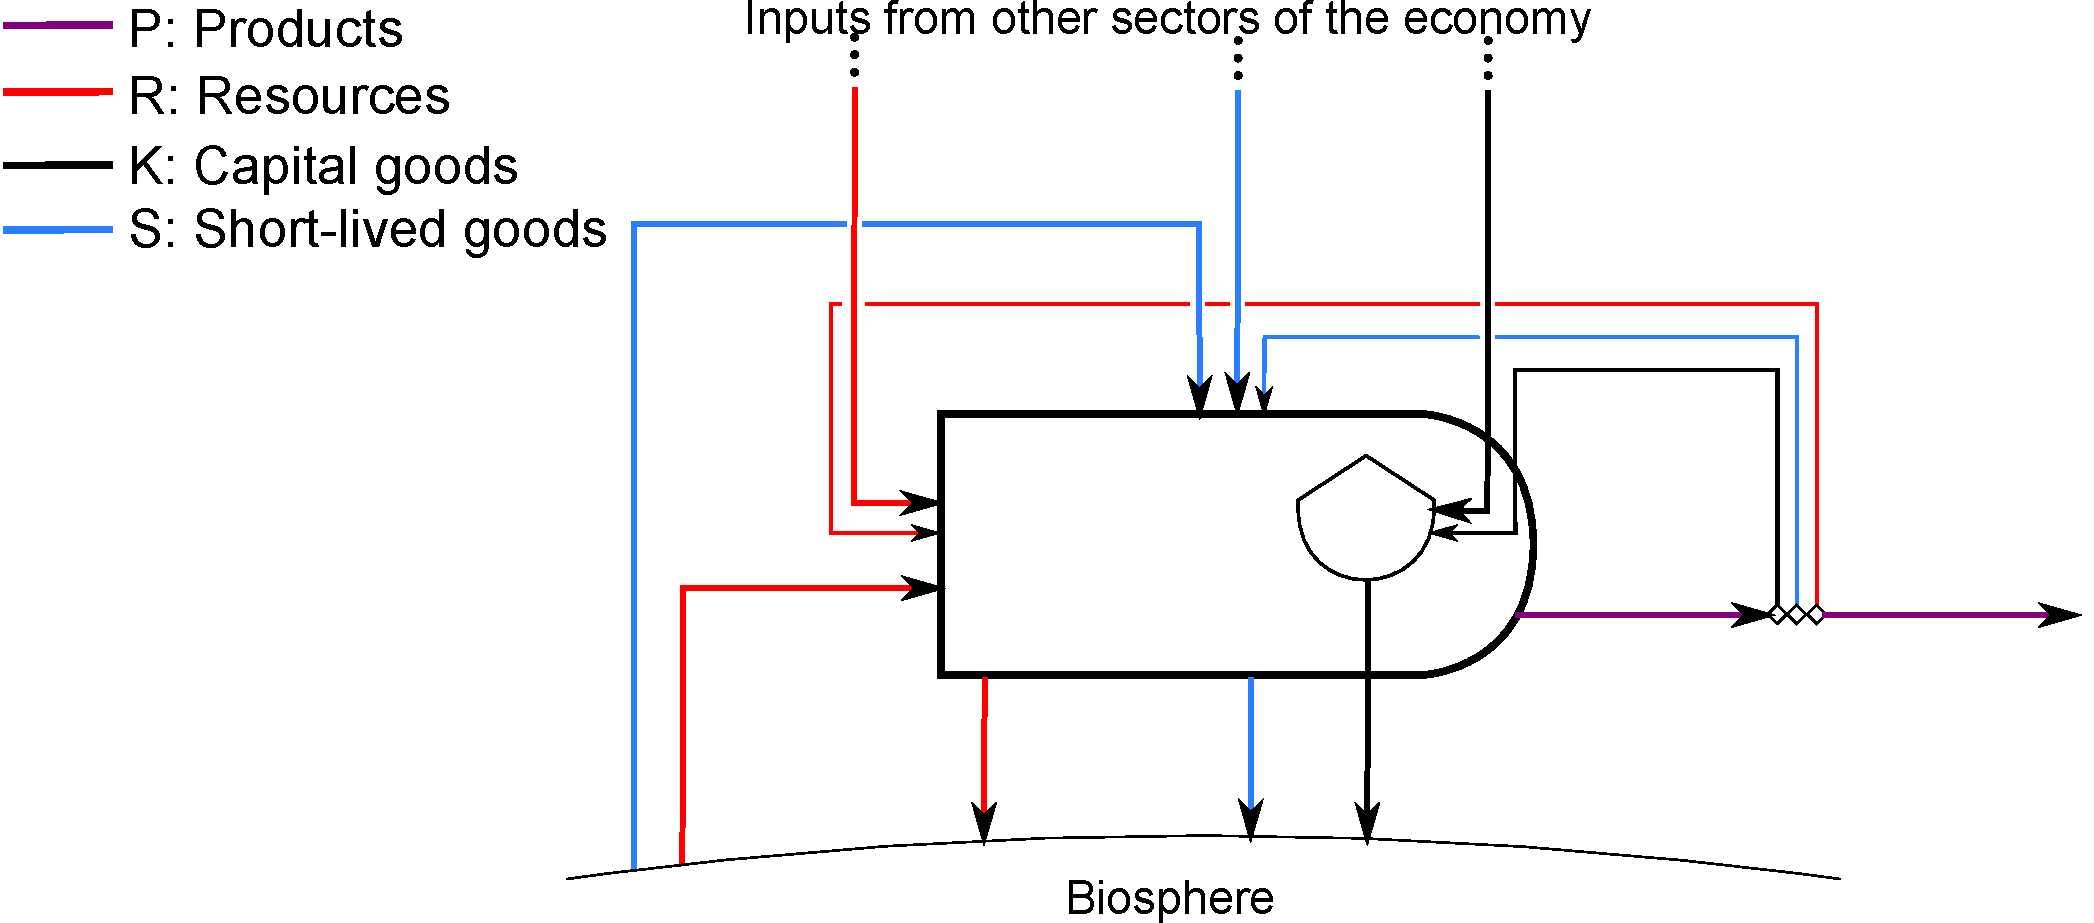
\includegraphics[width=\linewidth]{Part_1/Chapter_Materials/images/PERKS_basic_unit_materials.pdf}
\caption[Material flows into and out of a single sector 
of the economy]{Material flows into and out of 
a single sector of the economy. 
Resource flows ($\dot{R}$) enter the sector from the left 
and are embodied in products ($\dot{P}$) which leave from the right. 
Some waste resources are leave the sector at the 
bottom and are returned to the biosphere.
Short-lived material flows ($\dot{S}$) 
enter the sector from above and leave from below to return to the biosphere. 
Only capital stock ($\dot{K}$) may accumulate within the sector,
depicted by the storage tank.
These also enter the sector from above. 
Depreciated capital leaves the sector from below and is returned to the biosphere.}
\label{fig:PERKS_materials}
\end{figure}

Resource materials ($\dot{R}$)
enter the sector from the left.
They comprise those materials that are destined to be \emph{embodied} 
in the goods produced by the sector ($\dot{P}$), which leave from the right,
except for some proportion that is wasted.
All wastes depart from the bottom of the sector and are
returned to the biosphere. 
For example, sheet metal, rubber, and glass
(as well as many other materials) 
enter the automobile sector as resources 
and end up as material parts of the cars that are produced. 
Some fraction of these resources ($\dot{R}$) may not make it into the final product, 
such as trimming scrap from metal parts stamping, 
and may be either recycled internally, 
or wasted to the biosphere. 
In this material accounting framework, 
resource materials are not accumulated within a sector.

Short-lived goods ($\dot{S}$)
include those materials 
that are necessary for the production processes of a sector, 
but are neither accumulated within the sector, 
nor destined to be materially part of the product of the sector. 
They enter the sector from above and leave the sector from
below to return to the biosphere. 
Examples of these short-lived flows include energy resources, such as
the electricity needed to run automobile factories 
% including any contribution from labor, **** contribution from labor seems out of place here --MKH ****
and process water used by the sector. 
Resources and short-lived materials make up 
Georgescu-Roegen's ``flow'' elements\footnote{In
fact,
Georgescu-Roegen does not make a distinction between
resource flows (that are \emph{physically embodied}
in the product) and other flows necessary to support production
of the product.
}~\cite{G-R1970} 
or Daly's ``material causes.''~\cite{Daly2006}

Many of the material flows into the sector, 
such as production equipment,
are necessary for the continued operation of a sector 
but are not counted as short-lived goods, 
because the operation of the sector is dependent 
upon the accumulation 
of these materials within the sector. 
Such flows are counted as capital goods ($K$).
Capital flows ($\dot{K}$) also enter from above, 
but are stored within the sector 
(represented by a storage tank) 
and are returned to the biosphere as 
physical capital depreciation.
Examples of these capital flows would be the factory and office buildings or
manufacturing equipment within the automobile industry.
We assume (for simplicity) that there is no re-use of capital stock
by other sectors of an economy,
e.g.\ resale of vehicles or other equipment after depreciation,
or recycling of material from capital stock into other goods,
e.g.\ scrap metal. 
The issue of recycling is discussed in greater detail in
Section~\ref{sec:recycling}.

All products ($\dot{P}$) leave to the right of the sector. 
A fraction of the $\dot{P}$ flow may be returned 
to the sector as self-consumption, 
accounted either as resources destined 
to be embodied in the product ($\dot{R}$), 
as short-lived materials ($\dot{S}$), 
or as capital goods~($\dot{K}$).
The remainder flows to other sectors within the economy 
or to Final Consumption~(1). 
In this material accounting framework, 
energy may be accounted as either 
an $\dot{R}$ flow or an $\dot{S}$ flow.
An example of energy as an $\dot{R}$ flow is crude oil 
to be converted into gasoline within a refinery: 
the resource inflow (crude oil) is
\emph{literally} embodied within the out-flowing product (gasoline).
An example of energy as an $\dot{S}$ flow is electricity
used by an automobile factory: the resource inflow (electrons)
is not embodied \emph{literally} in the out-flowing product (automobiles).
Similarly, the coal or natural gas flowing into a
power plant is accounted as an $\dot{S}$ flow, 
because the incoming chemical elements (carbon and hydrogen) \emph{do
not} depart the plant as the product.  
(The product of a power plant is electrons that ``travel'' through
electricity transmission lines.)
We also set up another material flow,
that of \emph{wastes} ($\dot{W}$) which include both
resource and short-lived goods flowing to the biosphere from sector $j$, 
such that:

\begin{equation}
\dot{W}_{j0} =  \dot{R}_{j0} + \dot{S}_{j0}
\end{equation}

This waste flow will be useful later in Section~\ref{sec:Embodied_Energy_Example_C}.
We now track these material flows through some model economies.

%%%%%%%%%% Materials: Example A %%%%%%%%%%
\section{Example~A: single-sector economy} % chktex 13
\label{sec:A_materials}
%%%%%%%%%%

Our first example looks at the case where 
all processes within the economy occur within
one sector---Society (1)---which exchanges materials 
with the Biosphere~(0) as depicted in
Figure~\ref{fig:A_materials}.  
%We do not distinguish between production and consumption.

\begin{landscape}
\begin{figure}[!ht]
\centering{}
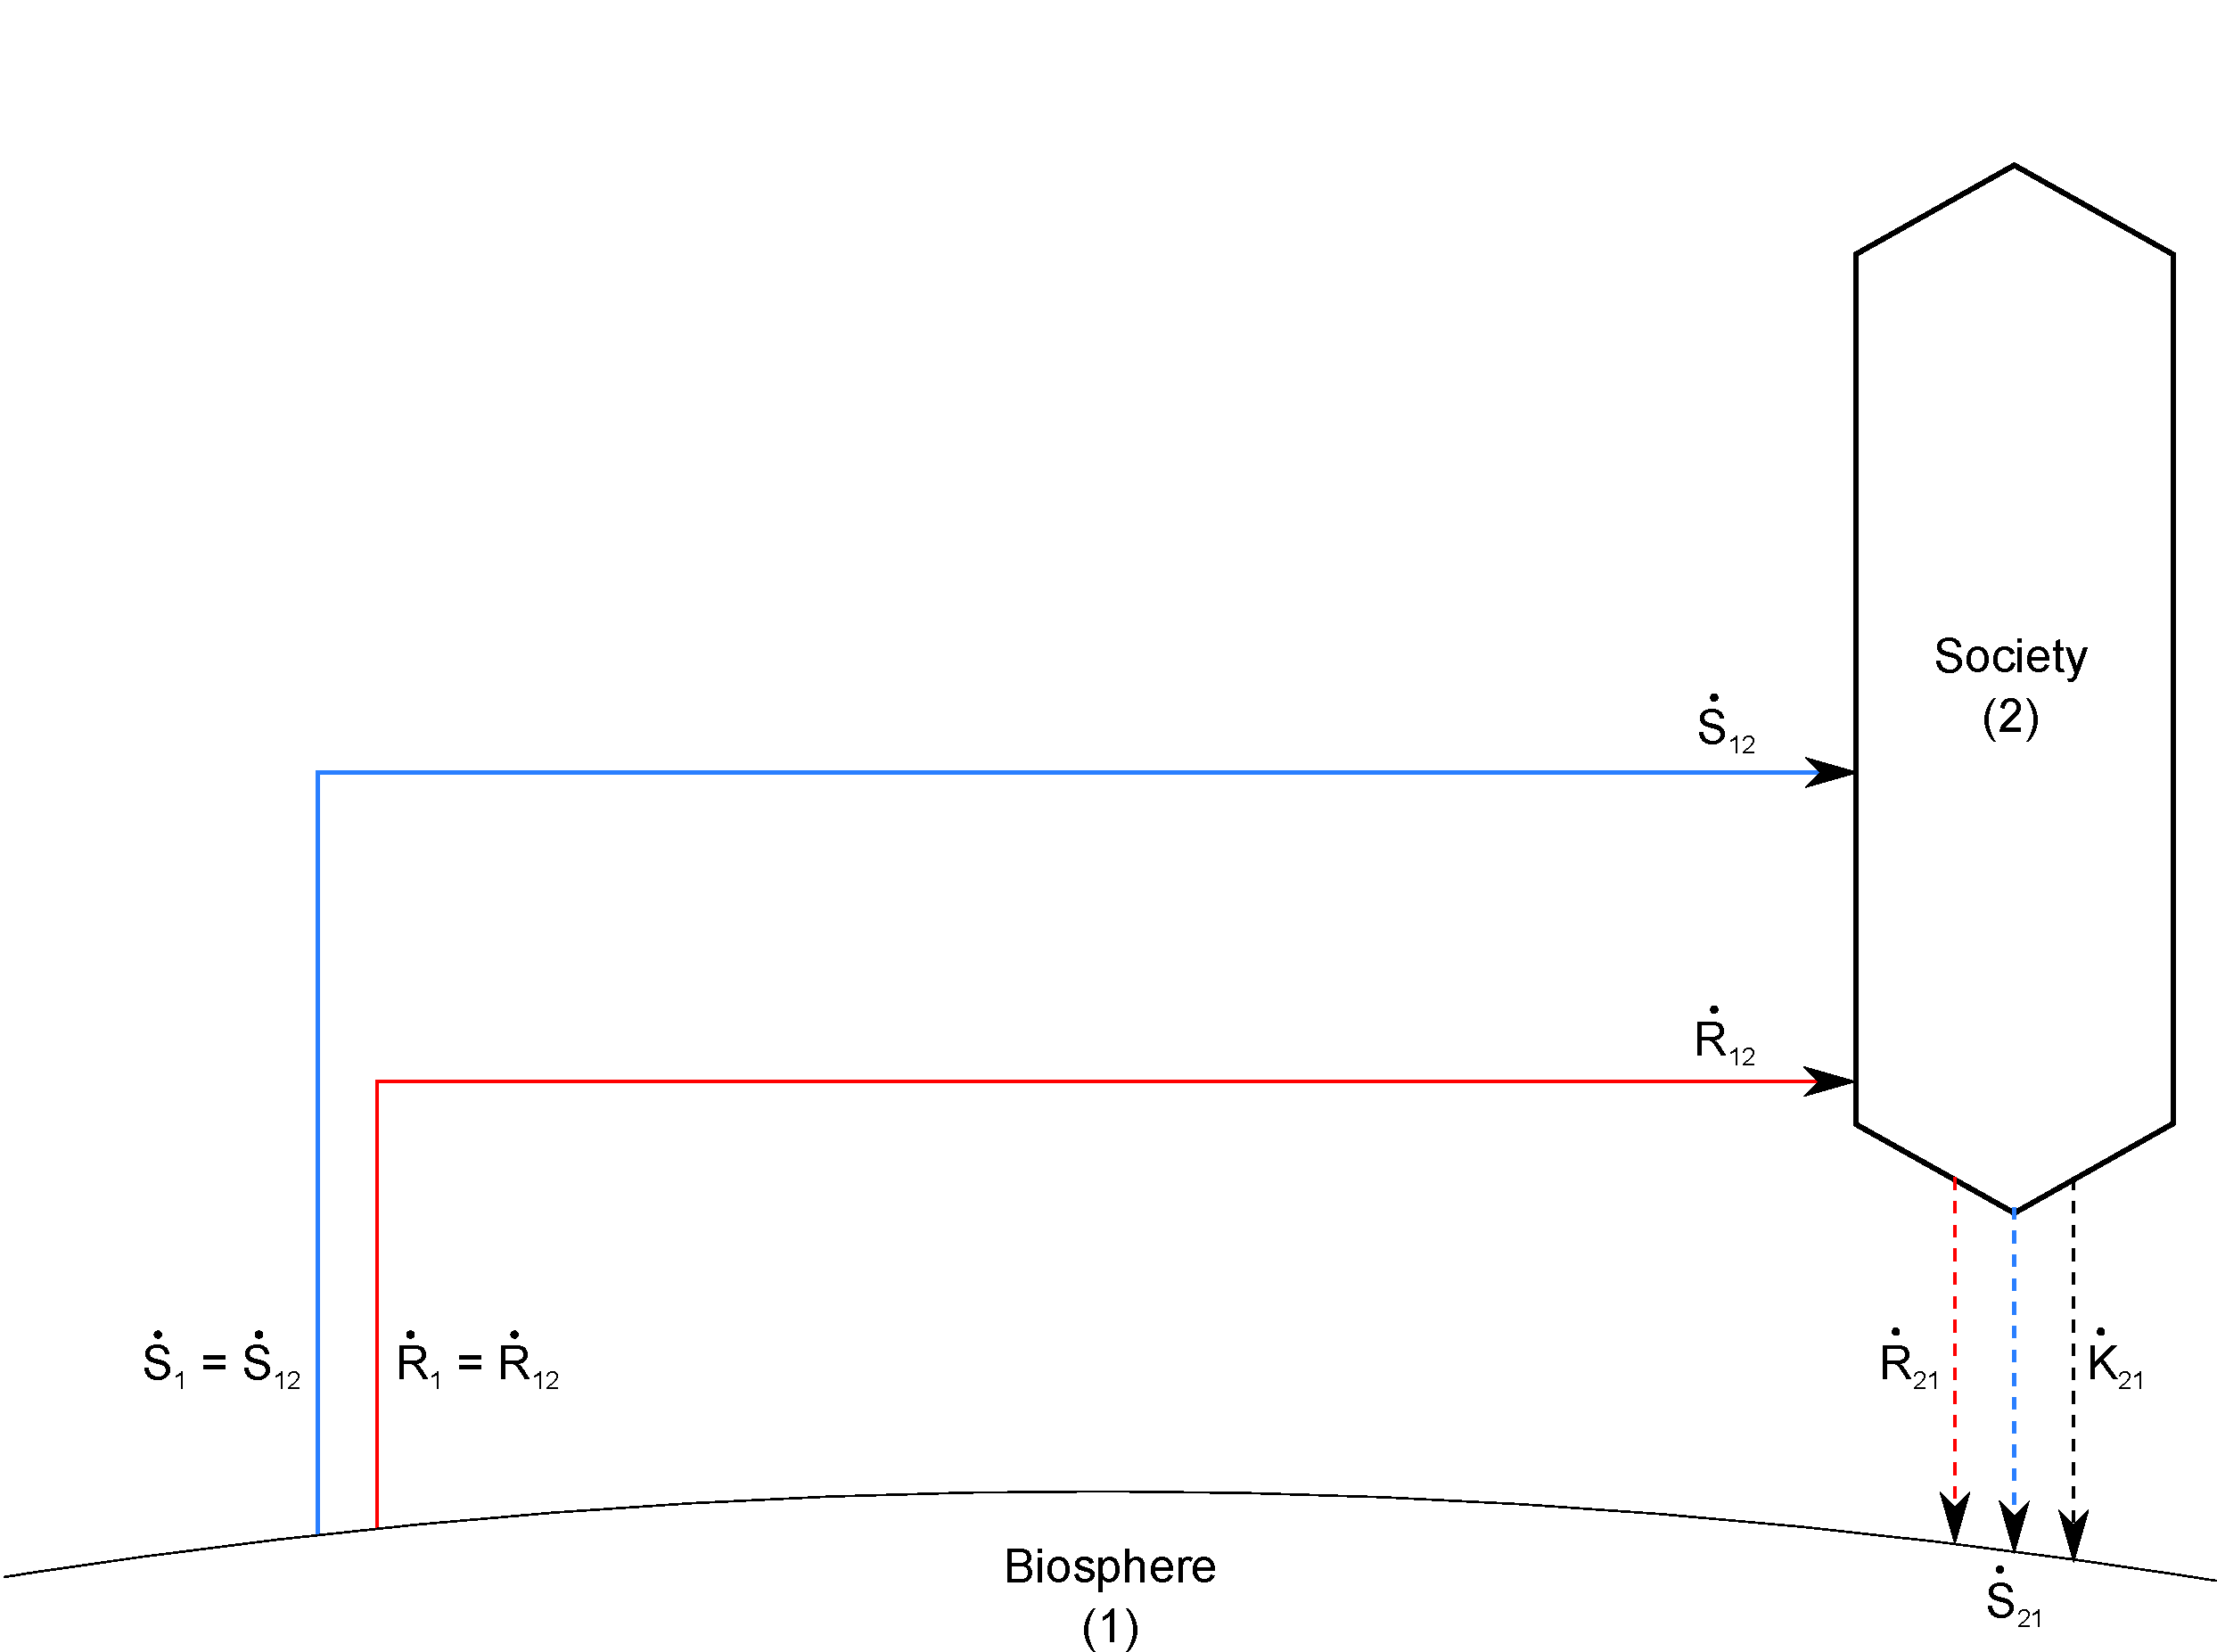
\includegraphics[width=0.8\linewidth]{Part_1/Chapter_Materials/images/1_sector_materials.pdf}
\caption[Flows of materials for a one-sector economy]{Flows of materials 
for a one-sector economy. 
Resources ($\dot{R}_{01}$) and short-lived materials 
($\dot{S}_{01}$) flow into the Society (1) 
from the Biosphere~(0). Waste resources 
($\dot{R}_{10}$) short-lived materials/goods 
($\dot{S}_{10}$) and capital goods
($\dot{K}_{10}$) are returned to the biosphere.}
\label{fig:A_materials}
\end{figure}
\end{landscape}

Resources, or perhaps more accurately raw materials
($\dot{R}_{01}$), such as crude oil or iron ore, 
and short-lived materials ($\dot{S}_{01}$), 
such as oxygen or water that flow 
\emph{through} economic processes but are not 
literally \emph{embodied} within the output, 
flow into Society (1) from the 
Biosphere~(0).\footnote{Double 
	subscripts on quantities
	(e.g., $\dot{R}_{ij}$) indicate a flow 
	from sector $i$ to sector $j$. 
	The first index always indicates the sector \emph{from} which a quantity flows, 
	and the second index indicates the sector \emph{to} which a quantity flows.
	Single subscripts on quantities such as
	$K$ can mean one of two things: 
	$\dot{K}_{j}$ (with a dot to indicate a flow) refers to 
	the outflow of capital from sector $j$, 
	whereas $K_{j}$ (without the dot) 
	denotes the capital stock of sector $j$.
	} 
These materials are processed within the economy 
into products ($\dot{P}_{1}$) consisting of 
resource goods ($\dot{R}_{11}$), 
short-lived goods ($\dot{S}_{11}$), 
and capital goods ($\dot{K}_{11}$)
which are able to be accumulated at some rate 
$\frac{\mathrm{d}K_{1}}{\mathrm{d}t}$ 
within the stock of materials within society.\footnote{See
	Section~\ref{sec:people_as_stock} for more discussion on
	the inclusion of human beings as societal capital stock.
	}
Waste resources ($\dot{R}_{10}$) and 
used short-lived materials/goods ($\dot{S}_{10}$)
are returned to the biosphere
without accumulating in Society~(1). 
Capital goods are returned to the biosphere
when they are physically depreciated ($\dot{K}_{10}$).

Drawing control volumes around both the 
Biosphere~(0) and Society~(1)
in Figure~\ref{fig:A_materials}, 
we can construct material accounting equations,
such that:

\begin{align} \label{eq:A_CV_0}
	\frac{\mathrm{d}R_0}{\mathrm{d}t}		
	+	\frac{\mathrm{d}S_0}{\mathrm{d}t}
	+	\frac{\mathrm{d}K_0}{\mathrm{d}t}			&	
	=	\dot{R}_{10}		
	+	\dot{S}_{10}	
	+	\dot{K}_{10}											
	-	\dot{R}_{0}											
	-	\dot{S}_{0}													\\
\label{eq:A_CV_1}
	\frac{\mathrm{d}R_{1}}{\mathrm{d}t}
	+ \frac{\mathrm{d}S_{1}}{\mathrm{d}t}
	+ \frac{\mathrm{d}K_{1}}{\mathrm{d}t}		&
	= \dot{R}_{01} 
	+ \dot{S}_{01} 
	+ \dot{R}_{11}
	+ \dot{S}_{11}
	+ \dot{K}_{11}
	- \dot{P}_{1}				
	- \dot{R}_{10}				
	- \dot{S}_{10}				
	- \dot{K}_{10}.
\end{align}

Because mass is conserved, we find that:

\begin{align} 
\label{eq:A_R0}
	\dot{R}_{0}				&
	= \dot{R}_{01},			\\
\label{eq:A_S0}
	\dot{S}_{0}				&
	= \dot{S}_{01},			\\
\label{eq:A_P1}
	\dot{P}_{1} 			&
	= \dot{R}_{11} 
	+ \dot{S}_{11}
	+ \dot{K}_{11},	
\end{align}

% \noindent{}such that Equations~\ref{eq:A_CV_0}~and~\ref{eq:A_CV_1} 
% become:

% \begin{align} \label{eq:A_CV_0a}
% 	\frac{\mathrm{d}R_0}{\mathrm{d}t}		
% 	+	\frac{\mathrm{d}S_0}{\mathrm{d}t}
% 	+	\frac{\mathrm{d}K_0}{\mathrm{d}t}		&	
% 	=	\dot{R}_{10}		
% 	+	\dot{S}_{10}	
% 	+	\dot{K}_{10}											
% 	-	\dot{R}_{01}											
% 	-	\dot{S}_{01}								\\
% \label{eq:A_CV_1a}
% 	\frac{\mathrm{d}R_{1}}{\mathrm{d}t}
% 	+ \frac{\mathrm{d}S_{1}}{\mathrm{d}t}
% 	+ \frac{\mathrm{d}K_{1}}{\mathrm{d}t}		&
% 	= \dot{R}_{01} 
% 	+ \dot{S}_{01} 
% 	- \dot{R}_{10}				
% 	- \dot{S}_{10}				
% 	- \dot{K}_{10}.
% \end{align}

Clearly, $\dot{R}_{01} \neq \dot{R}_{10}$ 
because some resources are converted into
short-lived goods ($\dot{S}_{11}$) or man-made capital ($\dot{K}_{11}$)
and are only returned to the biosphere as either
$\dot{S}_{10}$ or $\dot{K}_{10}$, respectively. 
Hence,
we may say that:

\begin{equation}\label{eq:A_dR0_neq_0}
	\frac{\mathrm{d}R_0}{\mathrm{d}t}
	= \dot{R}_{10}
	- \dot{R}_{01}
	\neq 0.
\end{equation}

Similarly, we know that
$\dot{S}_{01} \neq \dot{S}_{10}$.\footnote{While
this inequality may be true in theory,
it may be that in practice,
the large amount of material,
e.g.\ water or oxygen,
that passes straight through the economy ``unaffected,''
i.e.\ without being embodied in products,
is very large compared to the additional flow of short-lived goods
produced within the economy,
i.e.\ $\dot{S}_{11} << \dot{S}_{01}$.
}
%such that:
%
%\begin{equation}\label{eq:A_dS0_neq_0}
%	\frac{\mathrm{d}S_0}{\mathrm{d}t}
%	= \dot{S}_{10}
%	- \dot{S}_{01}
%	\neq 0.
%\end{equation}

%****BRH says, shouldn't this word be
%"accounting" -- not accumulation -- given that is what we
%called it in the sentence introducing eq. 2.4. Or, should we change "accounting" above to accumulation?
%Or, are they synonyms? And, aren't there two of these equations? 2.4 and 2.5? I added a separate
%label for eqn. 2.5**** MIK - Agreed, changed to 'material balance'

In this framework, neither resources ($R$) 
nor short-lived goods ($S$) accumulate 
within economic sectors, 
so we may state:

\begin{align}\label{eq:A-dS_1/dt_zero}
	\frac{\mathrm{d}R_1}{\mathrm{d}t}				&
	= 0,																	\\
	\frac{\mathrm{d}S_1}{\mathrm{d}t}				&
	= 0.
\end{align}

% \noindent{}which means that 
% Equations~\ref{eq:A_CV_0a}~and~\ref{eq:A_CV_1a}
% become:

% \begin{align}\label{eq:A_CV_0b}
% 	\frac{\mathrm{d}R_0}{\mathrm{d}t}		
% 	+	\frac{\mathrm{d}S_0}{\mathrm{d}t}
% 	+	\frac{\mathrm{d}K_0}{\mathrm{d}t}		&	
% 	=	\dot{R}_{10}		
% 	+	\dot{S}_{10}	
% 	+	\dot{K}_{10}											
% 	-	\dot{R}_{01}											
% 	-	\dot{S}_{01}								\\
% 	\label{eq:A_CV_1b}
% 	\frac{\mathrm{d}K_{1}}{\mathrm{d}t}		&
% 	= \dot{R}_{01} 
% 	+ \dot{S}_{01} 
% 	- \dot{R}_{10}				
% 	- \dot{S}_{10}				
% 	- \dot{K}_{10}.										
% \end{align}

% Equation~\ref{eq:A_CV_1b} indicates that the accumulation 
% of capital
% within society is the imbalance 
% between the flow of materials pulled from the biosphere
% ($\dot{R}_{01} + \dot{S}_{01}$) and the 
% flow rate of materials disposed back to the biosphere 
% ($\dot{R}_{10} + \dot{S}_{10} + \dot{K}_{10}$). 

Because the only ``capital'' that accumulates 
in the biosphere
is that which is a waste flow 
(capital depreciation)
from the economy,
(worn-out machines in the scrap yard),
we may say that:

\begin{equation} \label{eq:A_K0_balance}
	\frac{\mathrm{d}K_{0}}{\mathrm{d}t}		
	= \dot{K}_{10}
\end{equation}

Looking deeper at flows of resources and short-lived goods,
we can make some further observations. 
Imagine following a kilogram of coal on its journey through the economy. 
It is pulled out of the earth as part of flow $\dot{R}_{01}$. 
It enters the economy and while most 
is transformed into useful
products (part of $\dot{P}_{1}$) some (hopefully small)
fraction is wasted ($\dot{R}_{10}$).
Some of the coal is destined for electricity generation
and so re-enters the economy as part of flow $\dot{S}_{11}$,
because the coal is \emph{not physically embodied}
in the electricity and leaves the economy
(in the form of carbon dioxide and ash)
as part of flow $\dot{S}_{10}$.
Some of the coal is destined for metallurgical processes 
(such as the production of steel)
and so re-enters the economy within flow $\dot{R}_{11}$,
because the carbon in the coal ends up 
\emph{physically embodied} within the steel in flow $\dot{P}_{1}$.
Again,
some of the coal is wasted (maybe within slag), 
leaving the economy as flow $\dot{R}_{10}$.
The steel may re-enter the economy as part of
the resource flow $\dot{R}_{11}$ and be manufactured
into steel products (maybe a car) to leave as part of
flow $\dot{P}_{1}$
(again some being discharged within $\dot{R}_{10}$).
At this point the carbon 
(within the steel, within the car)
re-enters the economy as part of flow $\dot{K}_{11}$
and is accumulated within stock $K_{1}$.
Here it sits until such time as it is depreciated,
to leave the economy bound up in flow $\dot{K}_{10}$.
In summary, we may say that short-lived materials flow 
``straight through'' the economy and end up in the biosphere. 
 Resources are destined
to end up either physically embodied within products or waste ``resources.''
They cycle through the economy,
entering and re-entering,
until they are turned either into short-lived goods,
whereupon they flow ``straight through'' into the biosphere,
or they are turned into capital good and accumulate.

As such,
we may state that:

\begin{align}
% \label{eq:A_R1_balance}
	\frac{\mathrm{d}R_1}{\mathrm{d}t}		&
	= \dot{R}_{01}
	+ \dot{R}_{11}
	- \dot{P}_{1}
	- \dot{R}_{10}
	= 0,															\\
\label{eq:A_S1_balance}
	\frac{\mathrm{d}S_1}{\mathrm{d}t}		&
	= \dot{S}_{01}
	+ \dot{S}_{11}
	- \dot{S}_{10}
	= 0,
\end{align}

We may rearrange these equations in terms of
the important variable as:

\begin{align}
\label{eq:A_P1a}
	\dot{P}_{1}												&
	= \dot{R}_{01}
	+ \dot{R}_{11}
	- \dot{R}_{10}	,
\end{align}

\noindent{}and

\begin{align}
\label{eq:A_S11}
	\dot{S}_{11}											&
	= \dot{S}_{10}
	- \dot{S}_{01}.
\end{align}

Substituting Equations~\ref{eq:A_R0},~\ref{eq:A_S0}~and~\ref{eq:A_K0_balance}
into Equation~\ref{eq:A_CV_0} we obtain:

\begin{align}\label{eq:A_CV_0a}
	\frac{\mathrm{d}R_0}{\mathrm{d}t}		
	+	\frac{\mathrm{d}S_0}{\mathrm{d}t}		&	
	=	\dot{R}_{10}		
	+	\dot{S}_{10}	
	-	\dot{R}_{01}											
	-	\dot{S}_{01}.							% \\
%	\label{eq:A_CV_1c}
%	\dot{K}_{11}								&
%	= \dot{R}_{01} 
%	+ \dot{S}_{01} 
%	- \dot{R}_{10}				
%	- \dot{S}_{10}.
\end{align}





% **** Would we not also say that $\dot{S}_{01} = \dot{S}_{10}$? 
% The idea of the short-lived materials is that they are ``flow-through.''
% Think of water as the prototypical $\dot{S}$ flow. 
% The flow rate of water into society is probably very nearly equal
% to the flow rate of water out of society. 
% If this is right, the equations above simplify even further, right? 
% A counterpoint to this approach would be an argument that society
% ``makes'' $\dot{S}_{11}$ material for use by society (i.e.\ in the $\dot{P}_{11}$ flow).
% If society makes an $\dot{S}_{11}$, do we have
% $\dot{S}_{01} + \dot{S}_{11} = \dot{S}_{10}$?  --MKH ****
% I would definitely say that we are converting $\dot{R}_{01}$
% flows into $\dot{S}_{11}$ (and consequently $\dot{S}_{10}$ flows)
% in quite significant proportions, such as the large quantities of
% plastic packaging, paper,
% etc.\ waste that flows through but is never accumulated.
% How large this flow is (in mass terms) in comparison to,
% say water,
% is an open question. --MCD ****

Equation~\ref{eq:A_CV_0a} states that the rate of ``accumulation'' 
(or more accurately depletion) 
of natural capital~($R_{0}$ and $S_{0}$) 
is dependent on the rates at which society extracts these materials
from the biosphere ($\dot{R}_{01}$ and $\dot{S}_{01}$) and the rates
of disposal of waste materials back to the biosphere ($\dot{R}_{10}$ 
and $\dot{S}_{10}$).
Notice however, 
that although Equation~\ref{eq:A_CV_0a} 
is true for total mass of materials,
it does not account for the \emph{quality} of these materials.
Society relies heavily on extracted resources 
from naturally occurring accumulations that are 
far from equilibrium with their surroundings,
e.g.\ fossil fuel reservoirs or seams of high-grade ore. 
As these high quality material reserves are depleted 
and society must turn to lower grade reserves, 
more material must be processed 
(requiring the deployment of more productive capital)
in order to maintain the same level of 
production.\footnote{This theme 
	will be revisited in later sections,
	in relation to both energy~(direct energy in Chapter~\ref{chap:direct_energy}
	and embodied energy in Chapter~\ref{chap:embodied_energy}) and 
	value~(Chapter~\ref{chap:value}).
	}\cite{Mudd2010}

It is likely that the quality
of flow $\dot{R}_{01}$ is higher than flow $\dot{R}_{10}$ 
(e.g.\ overburden from mining operations). 
If this were not the case,
$\dot{R}_{10}$ could be easily substituted 
into the production process (i.e.\ recycled) thus
offsetting the need for primary resource extraction. 
The issue of recycling is discussed in more detail in 
Section~\ref{sec:recycling}.
The issue of material (and energy) quality 
is discussed in more detail in 
Section~\ref{sec:resource_quality_and_irreversibility}.

Substituting Equation~\ref{eq:A_S1_balance} 
into Equation~\ref{eq:A_CV_1}, we obtain:

\begin{align}\label{eq:A_CV_1b}
	\frac{\mathrm{d}K_{1}}{\mathrm{d}t}		&
	= \dot{R}_{01} 
	+ \dot{R}_{11}
	+ \dot{K}_{11}
	- \dot{P}_{1}				
	- \dot{R}_{10}				
	- \dot{K}_{10}.
\end{align}

Since we have two different formulations for $\dot{P}_{1}$,
represented by Equations~\ref{eq:A_P1} and~\ref{eq:A_P1a}, 
we may substitute either into Equation~\ref{eq:A_CV_1b}.
Substituting Equation~\ref{eq:A_P1a} 
into Equation~\ref{eq:A_CV_1b}, we obtain:

\begin{equation}\label{eq:A_CV_1c}
	\frac{\mathrm{d}K_{1}}{\mathrm{d}t}		
	= \dot{K}_{11}
	- \dot{K}_{10},
\end{equation}

\noindent{}which tells us that 
accumulation of capital in society~($K_{1}$)
is dependent only on 
inflows of capital into society~($\dot{K}_{11}$) 
and depreciation of capital 
to the biosphere ($\dot{K}_{10}$).

Substituting instead Equation~\ref{eq:A_P1} 
into Equation~\ref{eq:A_CV_1b}, we obtain:

 \begin{align}\label{eq:A_CV_1d}
	\frac{\mathrm{d}K_{1}}{\mathrm{d}t}		&
	= \dot{R}_{01} 
	- \dot{R}_{10}
	- \dot{S}_{11}
	- \dot{K}_{10}.
\end{align}

The last depreciation term~($\dot{K}_{10}$)
may be rewritten as the total stock
of man-made capital~($K_{1}$) 
multiplied by some depreciation rate~($\gamma_{K_{1}}$),\footnote{$\gamma_{K_{1}}$
	has units of inverse time, e.g.\ 1/year,
	and is inversely proportional to the average lifetime
	of man-made capital.}
where $\gamma_{K_{j}}$ is defined as:

\begin{equation}\label{eq:def_gamma}
\gamma_{K_{j}} \equiv \frac{\dot{B}_{j0}}{B_{j}},
\end{equation}

\noindent{}i.e.\ the depreciation 
\emph{per unit} of capital stock,\footnote{This
	depreciation term will be discussed in more depth in
	Sections~\ref{sec:depreciation_embodied}~and~\ref{sec:capital_accounting}.
	}
such that Equation~\ref{eq:A_CV_1d} may be rewritten:

 \begin{align}\label{eq:A_CV_1e}
	\frac{\mathrm{d}K_{1}}{\mathrm{d}t}		&
	= \dot{R}_{01} 
	- \dot{R}_{10}
	- \dot{S}_{11}
	- \gamma_{K_{1}}{K}_{1}.
\end{align}

We may rearrange Equation~\ref{eq:A_CV_1e} as:

 \begin{align}\label{eq:A_CV_1f}
	\dot{R}_{01} 
	- \dot{R}_{10}												&
	= 	\frac{\mathrm{d}K_{1}}{\mathrm{d}t}
	+ \dot{S}_{11}
	+ \gamma_{K_{1}}{K}_{1}.
\end{align}

Noticing that the left-hand side
of Equation~\ref{eq:A_CV_1f} is the negation 
of the right-hand side of Equation~\ref{eq:A_dR0_neq_0},
we may rewrite Equation~\ref{eq:A_CV_1f}
in terms of the accumulation
(or more accurately, depletion)
of natural resources: 

 \begin{align}\label{eq:A_CV_1g}
	- 	\frac{\mathrm{d}R_{0}}{\mathrm{d}t}	&
	= 	\frac{\mathrm{d}K_{1}}{\mathrm{d}t}
	+ \dot{S}_{11}
	+ \gamma_{K_{1}}{K}_{1}.
\end{align}

Equation~\ref{eq:A_CV_1g} tells us that depletion of
natural resources~$\left(-\frac{\mathrm{d}R_{0}}{\mathrm{d}t}\right)$
is used within society to:

\begin{itemize}
	\item build up societal capital stock 
	$\left(\frac{\mathrm{d}K_{1}}{\mathrm{d}t}\right)$,
	\item provide short-lived goods and energy to 
	run society ($\dot{S}_{11}$), and
	\item overcome depreciation
	($\gamma_{K_{1}}{K}_{1}$).
\end{itemize}
\noindent{}In other words,
the economy is completely dependent on stocks of natural resources
within the biosphere for all of these activities.
We now turn to a slightly more disaggregated model of the economy.


%%%%%%%%%% Materials: Example B %%%%%%%%%%
\section{Example~B: two-sector economy} % chktex 13
\label{sec:B_materials}
%%%%%%%%%%

In our second example B, we split society into two sectors: 
Production (2) and Final Consumption (1), 
as depicted in Figure~\ref{fig:B_materials}. 
Production~(2) makes all of the goods and services 
that are delivered to Final Consumption (1), 
as well as all of the intermediate goods that are not ``consumed'' 
by Final Consumption, 
but stay within Production, 
such as manufacturing equipment.

\begin{landscape}
\begin{figure}[!ht]
\centering
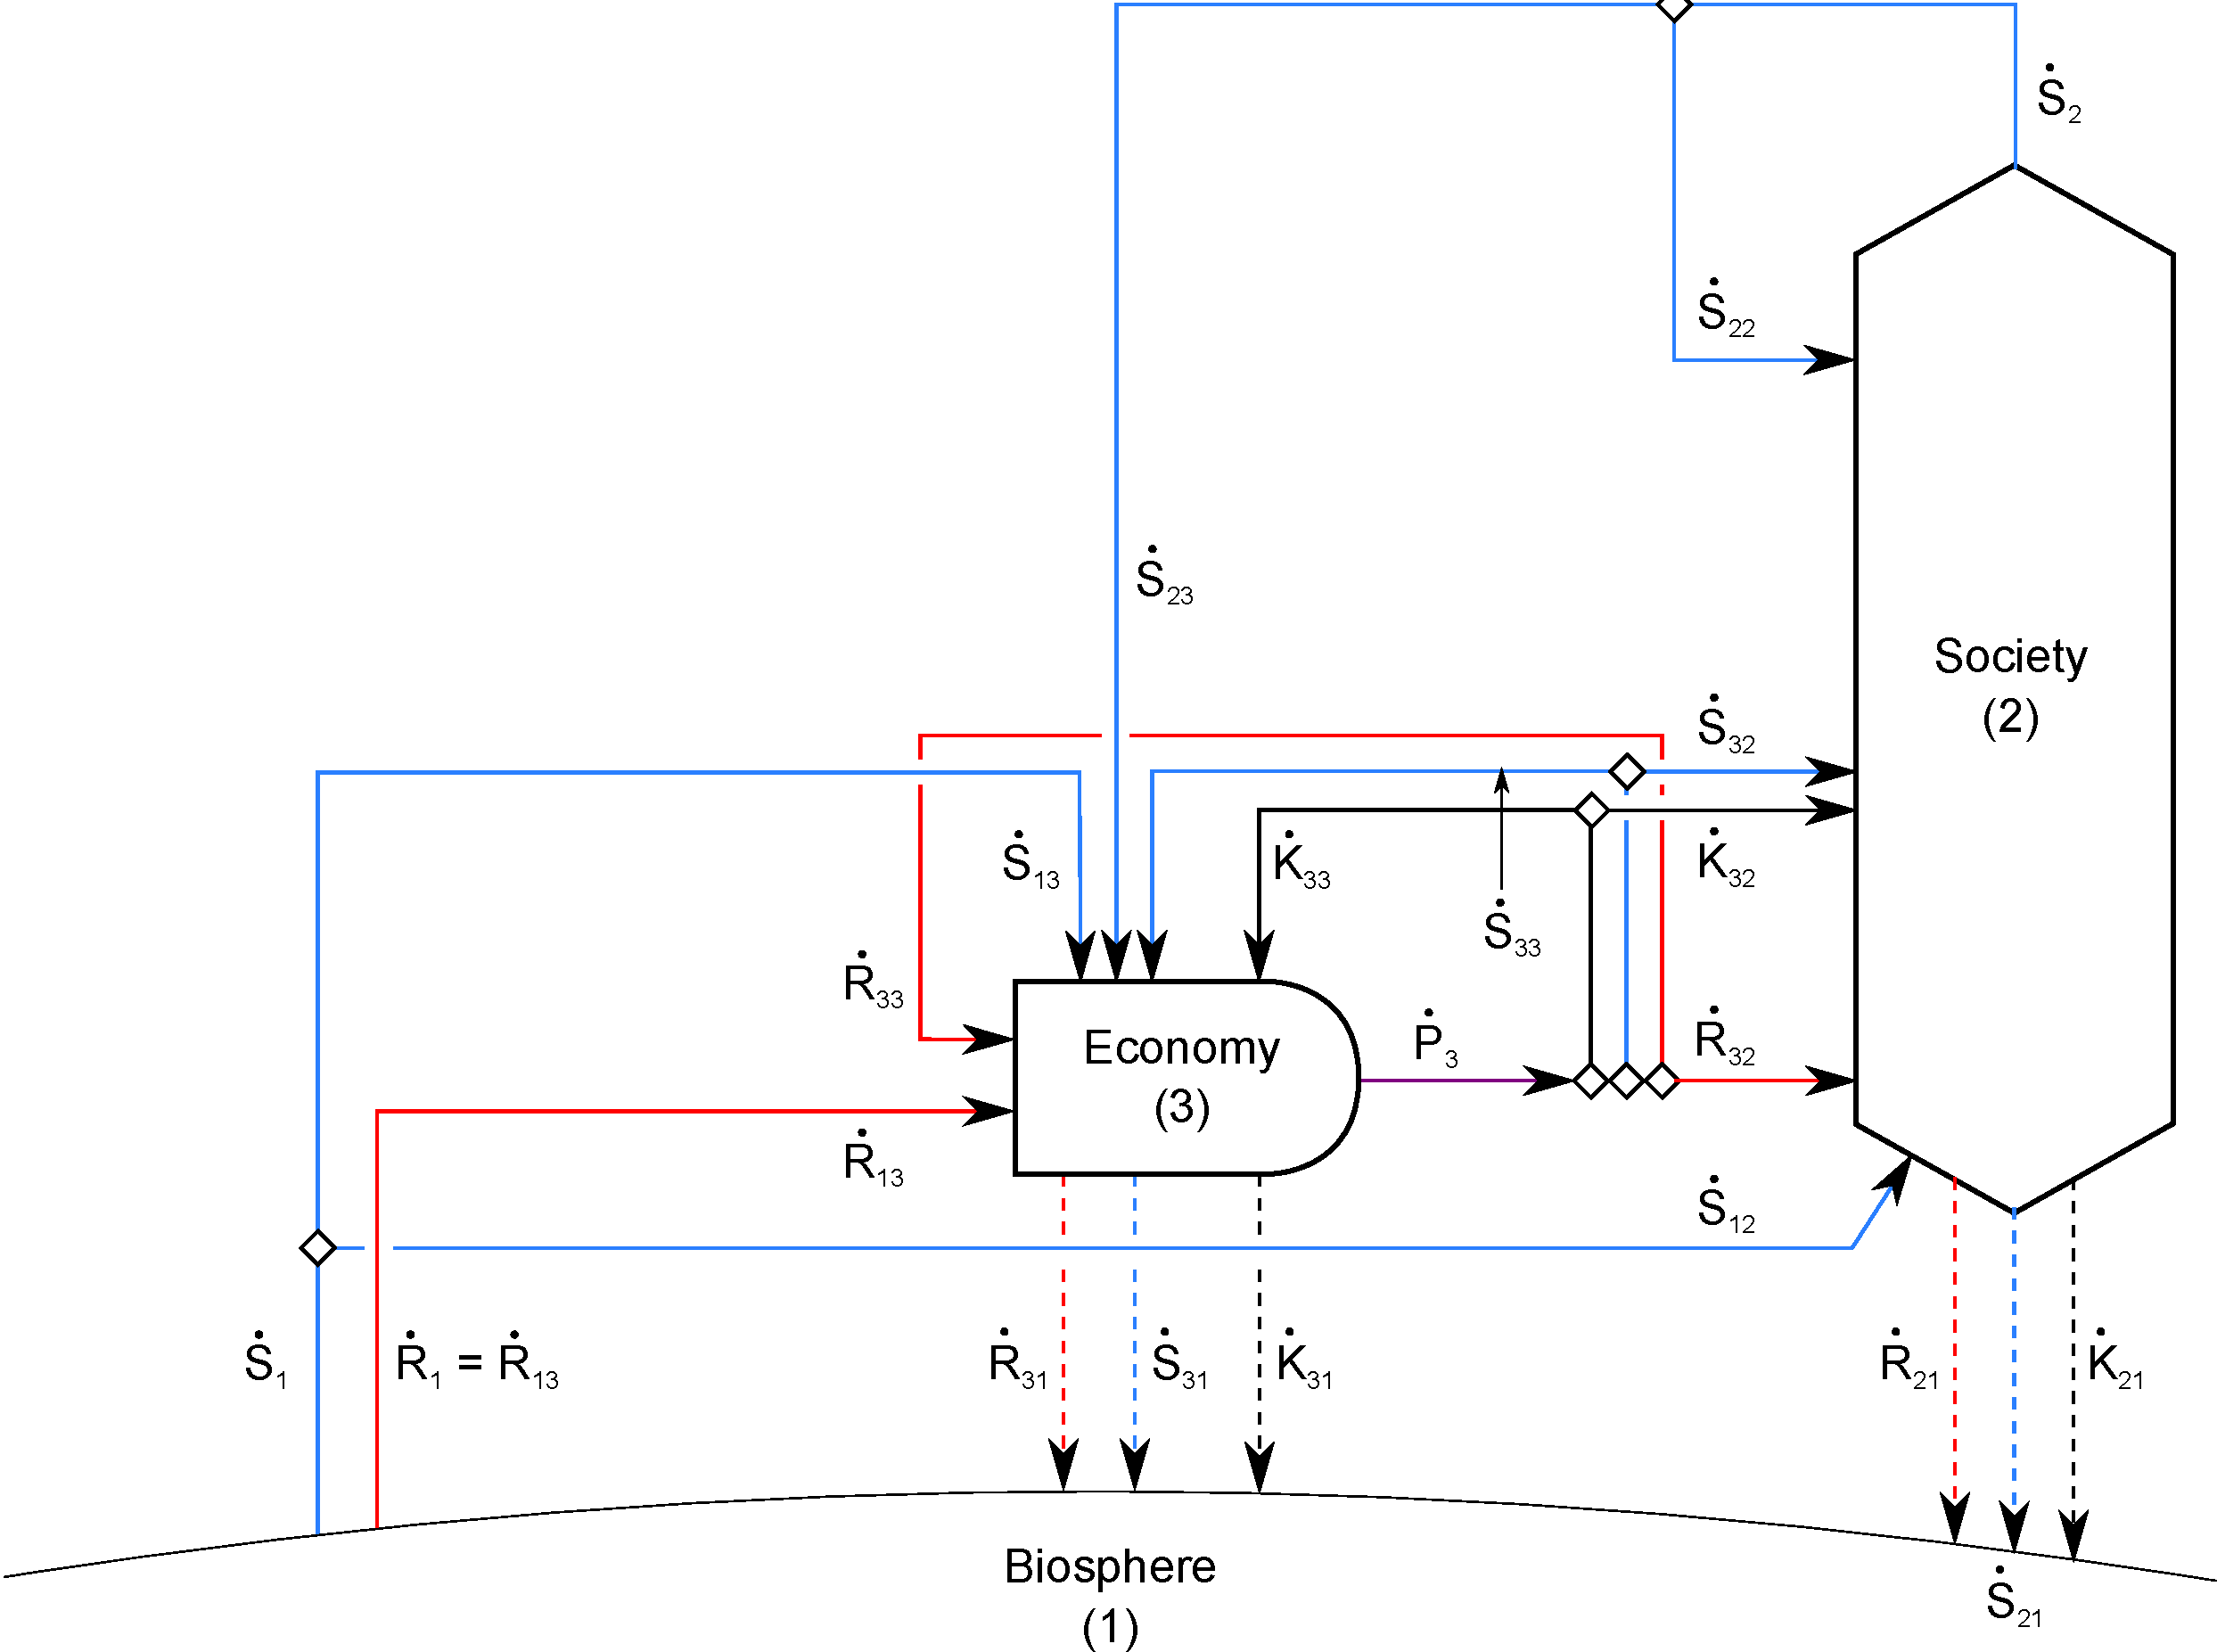
\includegraphics[width=0.8\linewidth]{Part_1/Chapter_Materials/images/2_sector_materials.pdf}
\caption[Flows of materials for a two-sector economy]{Flows of materials for a two-sector economy.}
\label{fig:B_materials}
\end{figure}
\end{landscape}

As can be seen in Figure~\ref{fig:B_materials}, 
Production~(2) resembles very closely the basic unit
shown in Figure~\ref{fig:PERKS_materials}. 
Resource flows from the biosphere ($\dot{R}_{02}$)
and those produced by Sector~(2) itself ($\dot{R}_{22}$) 
are \emph{transformed} into product flow
($\dot{P}_{2}$). 
Flows of short-lived goods ($\dot{S}$) 
and capital ($\dot{K}$) are required to
support this transformative process. 
Much of the product flow from ($\dot{P}_{2}$) 
enters Final Consumption~(1) as 
resource flows ($\dot{R}_{21}$), 
short-lived goods ($\dot{S}_{21}$) 
and capital goods ($\dot{K}_{21}$)
flows.

One point worth noting is that 
our flow of 
``capital goods''
into Final Consumption ($\dot{K}_{21}$) 
includes consumer durables and housing
in addition to typical items 
such as bridges and other public infrastructure.
We chose this approach because some goods 
(refrigerators, televisions, apartment blocks) 
may accumulate within Sector~(1)
and would be represented within flow 
$\dot{K}_{21}$, 
whereas other short-lived goods
(newspapers, plastic packaging, electricity) 
do not accumulate within Sector~1 and are represented by flow 
$\dot{S}_{21}$.

%\footnote{As has been mentioned elsewhere,
%this is a somewhat different conception of 
%``capital goods'' than is often used by economists, 
%whereby capital goods are used only within 
%productive sectors of the economy. 
%What we are here labeling as ``capital goods'' 
%might be termed \emph{consumer durables} by economists. 
% For our intention, consumer durables in society 
% serve the same purpose as capital equipment in the
% economy---they are necessary to support the goal 
% of the sector: production in one case
% and consumption in the other. [MAYBE REPHRASE AS ``production of goods in one case and production
% of labor in the other.'']}

There is also a product outflow 
from Final Consumption ($\dot{P}_{1}$), 
some of which is returned to Final Consumption~(1)
as resources ($\dot{R}_{11}$), 
short-lived goods ($\dot{S}_{11}$) 
and capital goods ($\dot{K}_{11}$) flows.\footnote{In actuality,
	both $\dot{R}_{11}$ and $\dot{S}_{11}$
	are zero,
	as will be discussed shortly.} 
%Short-lived goods ($\dot{S}_{12}$)
%flow from Final Consumption (1) 
%to Production (2) 
%associated with the flow of labor. 
There is no resource ($\dot{R}_{12}$) nor 
capital good ($\dot{K}_{12}$) flow from 
Final Consumption~(1) to Production~(2).
%This is because there is no resource flow associated
%with labor---it is not \emph{physically embodied}
%in products---and 
This is because the ``product'' of Final Consumption (1)
is labor services 
and because Final Consumption~(1) consumes, 
rather than produces, final goods. 
No resource materials flow from Final Consumption~(1) to be 
\emph{physically embodied} 
within the product output ($\dot{P}_{2}$), 
therefore $\dot{R}_{12} = 0$. 
Additionally, no capital \emph{goods} flow 
from Final Consumption~(1) to accumulate
within the production sector, 
therefore $\dot{K}_{12} = 0$.
% **** Rewrite this paragraph below ****
The flow of short-lived goods~($\dot{S}_{12}$) 
from Final Consumption~(1) to Production~(2)
represents labor,
specifically  the material flow 
associated with labor's energy 
which is used within the production sector.\footnote{We 
	assume that flow ($\dot{S}_{12}$) is the 
	adenosine triphosphate (ATP), 
	used as an energy
	carrier within the cells of organisms,
	which is consumed during activity (labor)
	} 

Resource flow $\dot{R}_{21}$ 
into Final Consumption represents 
the material flow that will be \emph{physically embodied} 
within the ``product'' of Final Consumption~(1)---human labor---which
is food produced by the agriculture industry

As in Example~A, 
we set control volumes around the biosphere
and our two economic sectors, 
such that the material accounting equations become:

\begin{align} 
\label{eq:B_CV_0}
	\frac{\mathrm{d}R_{0}}{\mathrm{d}t} 
	+ \frac{\mathrm{d}S_{0}}{\mathrm{d}t}	
	+ \frac{\mathrm{d}K_0}{\mathrm{d}t}		&
	=  \dot{R}_{10} + \dot{R}_{20} 
	+ \dot{S}_{10} + \dot{S}_{20} 
	+ \dot{K}_{10} + \dot{K}_{20} 
	- \dot{R}_{0} 
	- \dot{S}_{0} 							\\
\label{eq:B_CV_1}
	\frac{\mathrm{d}R_{1}}{\mathrm{d}t} 
	+ \frac{\mathrm{d}S_{1}}{\mathrm{d}t}	
	+ \frac{\mathrm{d}K_{1}}{\mathrm{d}t}	&
	=  \dot{R}_{11} 
	+ \dot{R}_{21}
	+ \dot{S}_{01} 
	+ \dot{S}_{11} 
	+ \dot{S}_{21}
	+ \dot{K}_{11}
	+ \dot{K}_{21}
	- \dot{P}_{1} 
	- \dot{R}_{10} 
	- \dot{S}_{10} 
	- \dot{K}_{10},							\\
\label{eq:B_CV_2}
	\frac{\mathrm{d}R_{2}}{\mathrm{d}t} 
	+ \frac{\mathrm{d}S_{2}}{\mathrm{d}t}
	+ \frac{\mathrm{d}K_{2}}{\mathrm{d}t}	&
	=  \dot{R}_{02} 
	+ \dot{R}_{22} 
	+ \dot{S}_{02} 
	+ \dot{S}_{12} 
	+ \dot{S}_{22} 
	+ \dot{K}_{22}
	- \dot{P}_{2}
	- \dot{R}_{20} 
	- \dot{S}_{20} 
	- \dot{K}_{20},
\end{align}

 %[WE NEED TO DISCUSS IF WE WANT TO ACCOUNT IT IN THIS WAY]
Because no resources flow directly to Final Consumption~(1)
from the Biosphere~(0),\footnote{A 
	counter-example to this assumption is 
	the production of food
	outside of the agricultural industry, 
	i.e.\ by households, 
	which may be large in agrarian economies.
	}
 we may say:

\begin{equation}\label{eq:B_R0}
	\dot{R}_{0} = \dot{R}_{02}.
\end{equation}

In contrast, 
short-lived materials \emph{do} flow directly to Final Consumption~(1) 
from the Biosphere~(0), 
for example the flow of photons in Sunlight or 
oxygen into car engines and lungs. 
We can redefine flow $\dot{S}_{0}$:
%and $\dot{S}_{1}$:

\begin{equation}\label{eq:B_S0}
	\dot{S}_{0} 
	= \dot{S}_{01} + \dot{S}_{02}.
\end{equation}

As in Example A, we may easily define 
the balance of resources ($\dot{R}$),
short-lived materials ($\dot{S}$) and
capital ($\dot{K}$) within the biosphere:

\begin{align}\label{eq:B_dR0}
	\frac{\mathrm{d}R_{0}}{\mathrm{d}t}	&
	= \dot{R}_{10}
	+ \dot{R}_{20}
	- \dot{R}_{02},										\\
\label{eq:B_dS0}
	\frac{\mathrm{d}S_{0}}{\mathrm{d}t}	&
	= \dot{S}_{10}
	+ \dot{S}_{20}
	- \dot{S}_{01}
	- \dot{S}_{02},										\\	
\label{eq:B_dK0}
	\frac{\mathrm{d}K_{0}}{\mathrm{d}t}	&
	= \dot{K}_{10}
	+ \dot{K}_{20}.
\end{align}

Because we are assuming that only man-made capital
(and not human beings themselves)
are accounted within the physical stock of 
Final Consumption\footnote{If
	we were assuming that the human population
	was accounted within $\dot{K}_{1}$,
	then the ``product'' of Final Consumption~(1) would be human beings
	(and the labor they provide),
	resource flow $\dot{R}_{11}$ would be material resources
	provided to human reproduction and
	``capital goods'' flow $\dot{K}_{11}$ would be material
	added to the human population stock. Again, 
	this issue is discussed in greater detail in 
	Section~\ref{sec:people_as_stock}.
}~($K_{1}$)
and that the ``product'' of Final Consumption~(1) is labor
(a short-lived material flow,~$\dot{S}$),
then we may also state that

\begin{align}
\label{eq:B_R11}
	\dot{R}_{11}				& 
	= 0,
\end{align}

\noindent{}since labor is not a resource flow---it
is not \emph{physically embodied} within products
produced within the production sector---and additionally that,

\begin{align}
\label{eq:B_K11}
	\dot{K}_{11}				& 
	= 0,
\end{align}
 
\noindent{}because all capital goods are produced within
the Production sector~(2).

% **** Are flows $\dot{R}_{11} = \dot{K}_{11} = 0$ *****
% **** Yes, they are, since we are assuming that
% $K_{1}$ includes only man-made capital, not humans
% and all capital manufacture occurs in 
% the production sector.

% [NOT SURE IF THIS IS TRUE IF WE THINK OF $\dot{R}_{12}$ AS FOOD AND $K_{1}$ 
% AS INCLUDING HUMANS\ldots 
% YES, I THINK $\dot{R}_{12}$ CAN BE TURNED INTO  $\dot{K}_{1}$ INTERNALLY, 
% AS THE ACCUMULATION OF (LITERAL) HUMAN CAPITAL, I.E. POPULATION]



From conservation of mass,
we can also define product flows
$\dot{P}_{1}$ and $\dot{P}_{2}$ as:.

\begin{align}
\label{eq:B_P1_def}
	\dot{P}_{1}				&
	= \dot{S}_{11}
	+ \dot{S}_{12},
\end{align}

\noindent{}and

\begin{align}
\label{eq:B_P2_def}
	\dot{P}_{2}				&
	= \dot{R}_{21}
	+ \dot{R}_{22}
	+ \dot{S}_{21}
	+ \dot{S}_{22}
	+ \dot{K}_{21}	 
	+ \dot{K}_{22}
\end{align}

\noindent Again, remembering that resources ($R$) 
and short-lived goods ($S$) do not accumulate 
within any sectors of the economy:

\begin{align}
\label{eq:dR_and_dS_zero}
	\frac{\mathrm{d}R_{1}}{\mathrm{d}t}			&
	= 0,																	\\
	\frac{\mathrm{d}R_{2}}{\mathrm{d}t} 			&
	= 0,																	\\
	\frac{\mathrm{d}S_{1}}{\mathrm{d}t} 			&
	= 0,
\end{align}

\noindent{}and

\begin{align}
	\frac{\mathrm{d}S_{2}}{\mathrm{d}t} 			&
	= 0.
\end{align}

As in Example~A,
we may also define the resource-product
and short-lived goods flows balances separately
for each of the sectors of the economy:

\begin{align}
	\frac{\mathrm{d}R_{1}}{\mathrm{d}t} 	&
	= \dot{R}_{21}
	- \dot{P}_{1}
	- \dot{R}_{10}
	= 0,															\\
\label{eq:B_dS1}
	\frac{\mathrm{d}S_{1}}{\mathrm{d}t} 	&
	= \dot{S}_{01}
	+ \dot{S}_{11}
	+ \dot{S}_{21}
	- \dot{S}_{10}
	= 0,															\\
	\frac{\mathrm{d}R_{2}}{\mathrm{d}t} 	&
	= \dot{R}_{02}
	+ \dot{R}_{22}
	- \dot{P}_{2}
	- \dot{R}_{20}
	= 0,
\end{align}

\noindent{}and

\begin{align}
\label{eq:B_dS2}
	\frac{\mathrm{d}S_{2}}{\mathrm{d}t} 	&
	= \dot{S}_{02}
	+ \dot{S}_{12}
	+ \dot{S}_{22}
	- \dot{S}_{20}
	= 0.
\end{align}

We may rearrange these equations in terms of
the important variables to obtain:

\begin{align}
\label{eq:B_P1a}
	\dot{P}_{1}												&
	= \dot{R}_{21}
	- \dot{R}_{10}											\\
\label{eq:B_S11}
	\dot{S}_{11}											&
	= \dot{S}_{10}
	- \dot{S}_{21},										\\
\label{eq:B_P2a}
	\dot{P}_{2}												&
	= \dot{R}_{02}
	+ \dot{R}_{22}
	- \dot{R}_{20},
\end{align}

\noindent{}and

\begin{align}
\label{eq:B_S22}
	\dot{S}_{22}											&
	= \dot{S}_{20}
	- \dot{S}_{02} 
	- \dot{S}_{12}.	
\end{align}


Substituting
Equations~\ref{eq:B_R0}-\ref{eq:B_dK0}
into Equation~\ref{eq:B_CV_0}, 
gives,

\begin{align} \label{eq:B_CV_0a}
	\frac{\mathrm{d}R_{0}}{\mathrm{d}t} 
	+ \frac{\mathrm{d}S_{0}}{\mathrm{d}t}		& 
	= \dot{R}_{10} + \dot{R}_{20} 
	+ \dot{S}_{10} + \dot{S}_{20} 
	- \dot{R}_{02} 
	- \dot{S}_{01}
	- \dot{S}_{02}.
\end{align}

Substituting Equations~\ref{eq:dR_and_dS_zero},~\ref{eq:B_dS1}~and~\ref{eq:B_dS2}
into Equations~\ref{eq:B_CV_1}~and~\ref{eq:B_CV_2},
respectively,
we obtain:

\begin{align} 
\label{eq:B_CV_1a}
	 \frac{\mathrm{d}K_{1}}{\mathrm{d}t}	&
	=  \dot{R}_{21}
	+ \dot{K}_{21}
	- \dot{P}_{1} 
	- \dot{R}_{10} 
	- \dot{K}_{10}
\end{align}

\noindent{}and

\begin{align}
\label{eq:B_CV_2a}
	\frac{\mathrm{d}K_{2}}{\mathrm{d}t}	&
	=  \dot{R}_{02} 
	+ \dot{R}_{22} 
	+ \dot{K}_{22}
	- \dot{P}_{2}
	- \dot{R}_{20} 
	- \dot{K}_{20},
\end{align}


As in Example~A,
we again have two definitions for $\dot{P}_{1}$
(Equations~\ref{eq:B_P1_def} and~\ref{eq:B_P1a})
and $\dot{P}_{2}$ 
(Equations~\ref{eq:B_P2_def} and~\ref{eq:B_P2a})
which may be substituted into
Equations~\ref{eq:B_CV_1a} and~\ref{eq:B_CV_2a},
respectively. 
Let us start by substituting Equations~\ref{eq:B_P1a} and~\ref{eq:B_P2a},
in which case we obtain:

\begin{align} 
\label{eq:B_CV_1b}
	 \frac{\mathrm{d}K_{1}}{\mathrm{d}t}	&
	= \dot{K}_{21}
	- \dot{K}_{10},
\end{align}

\noindent{}and

\begin{align}
\label{eq:B_CV_2b}
	\frac{\mathrm{d}K_{2}}{\mathrm{d}t}	&
	=  \dot{K}_{22}
	- \dot{K}_{20},
\end{align}

\noindent{}Equations~\ref{eq:B_CV_1b} and~\ref{eq:B_CV_2b} 
tell us that accumulation 
of man-made capital~($K$) in each sector~($j$)
is dependent only on inflows of capital goods 
into that sector~($\dot{K}_{2j}$) and 
depreciation of capital to the biosphere 
from that sector~($\dot{K}_{j0}$).

Now, substituting
Equations~\ref{eq:B_P1_def} and~\ref{eq:B_P2_def},
we obtain:

\begin{align} 
\label{eq:B_CV_1c}
	 \frac{\mathrm{d}K_{1}}{\mathrm{d}t}	&
	=  \dot{R}_{21}
	+ \dot{K}_{21}
	- \dot{S}_{11}
	- \dot{S}_{12} 
	- \dot{R}_{10} 
	- \dot{K}_{10},
\end{align}

\noindent{}and

\begin{align}
\label{eq:B_CV_2c}
	\frac{\mathrm{d}K_{2}}{\mathrm{d}t}	&
	=  \dot{R}_{02} 
	- \dot{R}_{21}
	- \dot{S}_{21}
	- \dot{S}_{22}
	- \dot{K}_{21}	 
	- \dot{R}_{20} 
	- \dot{K}_{20},
\end{align}

\noindent{}to which we may make the 
substitution of the depreciation term 
(as in Example~A) and rearrange 
to obtain:

\begin{align} 
\label{eq:B_CV_1d}
	- \dot{R}_{10} 	 										&
	 = \frac{\mathrm{d}K_{1}}{\mathrm{d}t}
	-  \dot{R}_{21}
	- \dot{K}_{21}
	+ \dot{S}_{11}
	+ \dot{S}_{12} 
	+ \gamma_{K_{1}}K_{1},
\end{align}

\noindent{}and

\begin{align}
\label{eq:B_CV_2d}
	\dot{R}_{02}
	- \dot{R}_{20} 											&
	= \frac{\mathrm{d}K_{2}}{\mathrm{d}t}	
	+ \left(\dot{R}_{21}
	+ \dot{S}_{21}
	+ \dot{K}_{21}\right)	 
	+ \dot{S}_{22}
	+ \gamma_{K_{2}}K_{2}.
\end{align}

Equation~\ref{eq:B_CV_2d} tells us that 
the resources extracted and used by 
the production sector~($\dot{R}_{02} - \dot{R}_{20}$)
are for the purposes of: 

\begin{itemize}
	\item{building up capital stock
	in the production sector
	$\left(\frac{\mathrm{d}K_{2}}{\mathrm{d}t}\right)$,}

	\item{providing goods 
	for Final Consumption
	$\left(\dot{R}_{21}
	+ \dot{S}_{21}
	+ \dot{K}_{21}\right)$,}

	\item{providing short-lived goods
	to support the 
	production sector ($\dot{S}_{22}$), and

	\item overcoming depreciation of production 
	capital stock ($\gamma_{K_{2}}K_{2}$).}
\end{itemize}

Adding Equations~\ref{eq:B_CV_1d}~and~\ref{eq:B_CV_2d} together,
we obtain:

\begin{align} 
	- \frac{\mathrm{d}R_{0}}{\mathrm{d}t}			&
	= \dot{R}_{02}
	- \dot{R}_{10}
	- \dot{R}_{20}									\nonumber	\\
\label{eq:B_CV_1and2}											&
	= \frac{\mathrm{d}K_{1}}{\mathrm{d}t}
	+ \frac{\mathrm{d}K_{2}}{\mathrm{d}t}
	+ \dot{S}_{11}
	+ \dot{S}_{12} 
	+ \dot{S}_{21}
	+ \dot{S}_{22}
	+ \gamma_{K_{1}}K_{1}
	+ \gamma_{K_{2}}K_{2}.
\end{align}

\noindent{}which tells us that
the depletion of natural resources
$\left(\frac{\mathrm{d}R_{0}}{\mathrm{d}t}\right)$
is used within the whole economy to:

\begin{itemize}
	\item{build up capital stock
	$\left(\frac{\mathrm{d}K_{1}}{\mathrm{d}t}
	+ \frac{\mathrm{d}K_{2}}{\mathrm{d}t}\right)$,}
	\item{produce short-lived goods
	($\dot{S}_{11}
	+ \dot{S}_{12} 
	+ \dot{S}_{21}
	+ \dot{S}_{22}$), and}
	\item{overcome depreciation
	$\left(\gamma_{K_{1}}K_{1}
	+ \gamma_{K_{2}}K_{2}\right)$.}
\end{itemize}

We now turn to a three-sector model of the economy
in order to generalize these results.


%%%%%%%%%% Materials: Example C %%%%%%%%%%
\section{Example C: three-sector economy} % chktex 13
\label{sec:C_materials}
%%%%%%%%%%

In Example~C, we differentiate between two production sectors, sector (2) produces energy
and sector (3) produces other goods and services, as depicted in Figure
\ref{fig:C_materials}.

\begin{landscape}
\begin{figure}[!ht]
\centering
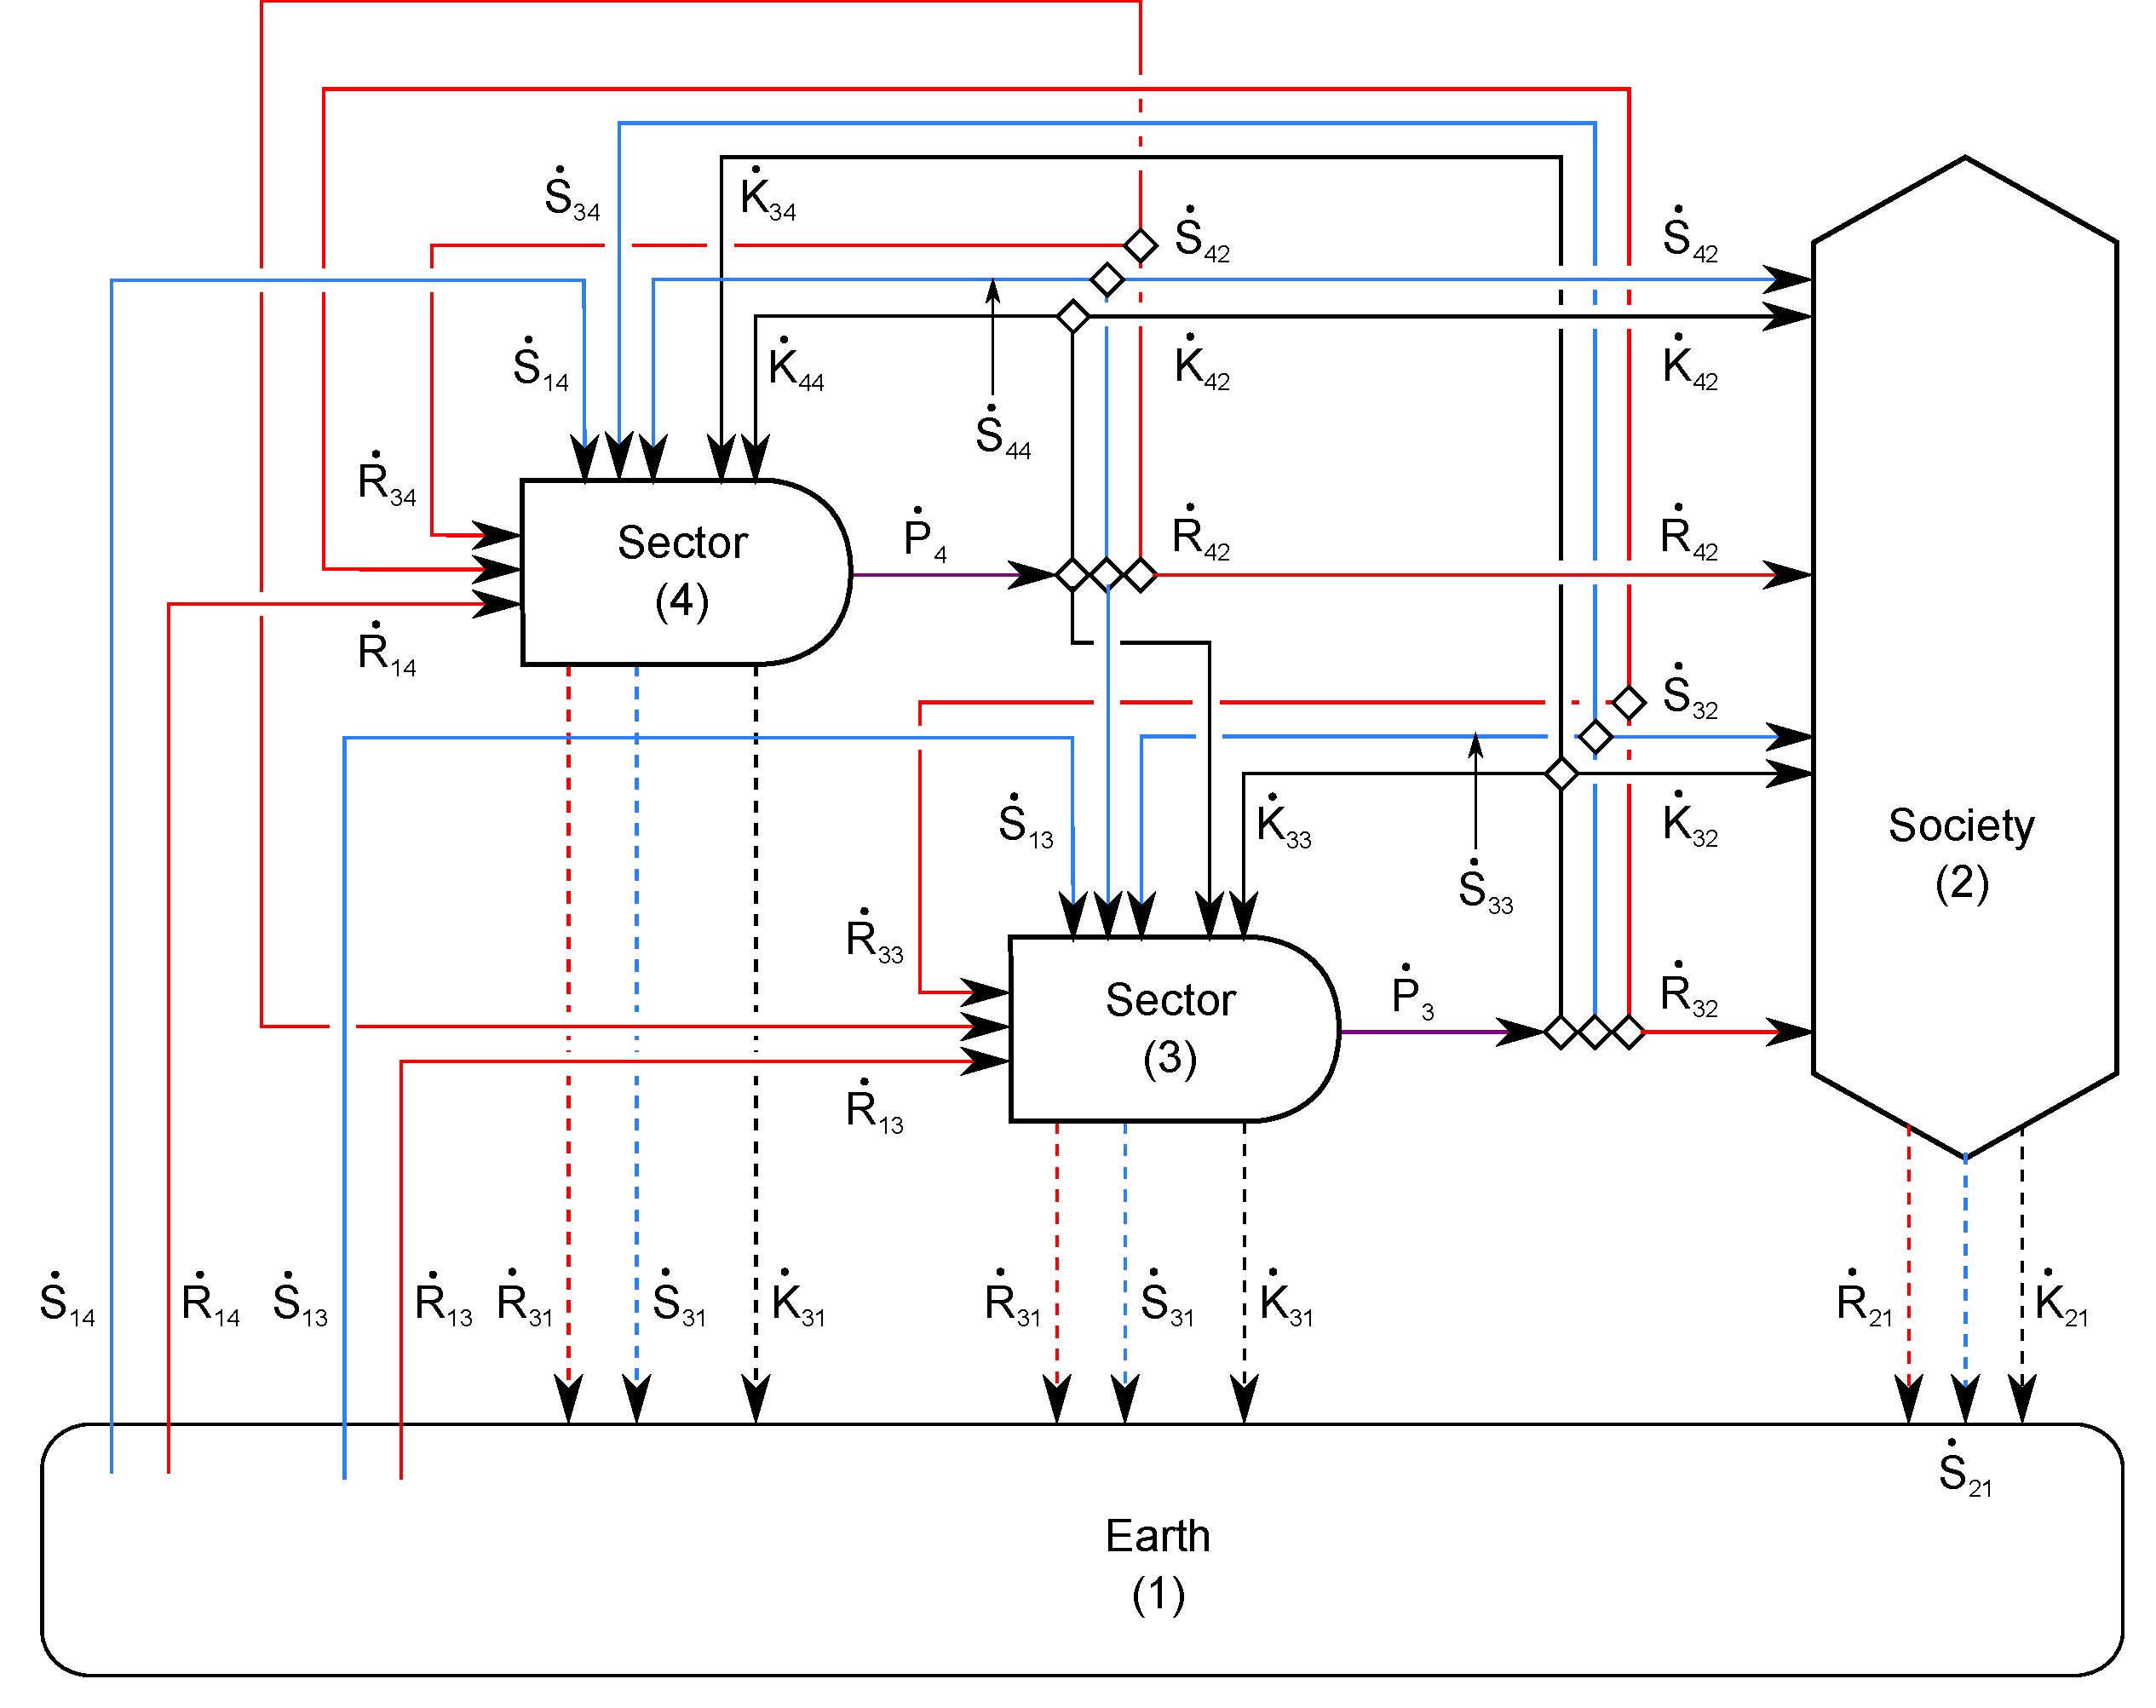
\includegraphics[width=0.8\linewidth]{Part_1/Chapter_Materials/images/3_sector_materials.pdf}
\caption[Flows of materials for a three-sector economy]{Flows of materials for a three-sector economy.}
\label{fig:C_materials}
\end{figure}
\end{landscape}

In this example, we will take a slightly different approach
than in the previous two examples. 
Instead of discerning whether or not certain flows exist
(asking for example,
``is there a flow of resources ($\dot{R}_{21}$) from
Energy~(2) to Final Consumption~(1)?''),
we shall account for all flows,
\emph{even if} those flows are zero.
In this way,
we may build up a completely general
framework for material accounting within an economy
of any size.

Accounting for the material flows 
into and out of the Biosphere
(0) gives the following equation:

\begin{align} \label{eq:C_CV_0}
	\frac{\mathrm{d}R_{0}}{\mathrm{d}t} 
	+ \frac{\mathrm{d}S_{0}}{\mathrm{d}t}	
	+ \frac{\mathrm{d}K_0}{\mathrm{d}t}		
	& =  \dot{R}_{10} + \dot{R}_{20} + \dot{R}_{30}
	+ \dot{S}_{10} + \dot{S}_{20} + \dot{S}_{30}
	+ \dot{K}_{10} + \dot{K}_{20} + \dot{K}_{30}
	- \dot{R}_{0} 
	- \dot{S}_{0},
\end{align}

\noindent{}which may be rewritten as:

\begin{align} \label{eq:C_CV_0_b}
	\frac{\mathrm{d}R_{0}}{\mathrm{d}t} 
	+ \frac{\mathrm{d}S_{0}}{\mathrm{d}t}	
	+ \frac{\mathrm{d}K_0}{\mathrm{d}t}		
	& =  \sum_{i = 1}^{3}\dot{R}_{i0}
	+ \sum_{i = 1}^{3}\dot{S}_{i0}
	+ \sum_{i = 1}^{3}\dot{K}_{i0}
	- \dot{R}_{0} 
	- \dot{S}_{0},
\end{align}

\noindent{}where the sum represents flows
into the biosphere from each of the other $i$ sectors.
Similarly, flows for the other sectors may be written:

\begin{align} \label{eq:C_CV_1}
	\frac{\mathrm{d}R_{1}}{\mathrm{d}t} 
	+ \frac{\mathrm{d}S_{1}}{\mathrm{d}t}	
	+ \frac{\mathrm{d}K_{1}}{\mathrm{d}t}		
	& =  \dot{R}_{01} 
	+ \dot{S}_{01}
	+ \sum_{i = 1}^{3}\dot{R}_{i1}
	+ \sum_{i = 1}^{3}\dot{S}_{i1}
	+ \sum_{i = 1}^{3}\dot{K}_{i1}
	- \dot{P}_{1}
	- \dot{R}_{10} 
	- \dot{S}_{10}
	- \dot{K}_{10},										\\
	\label{eq:C_CV_2}
	\frac{\mathrm{d}R_{2}}{\mathrm{d}t} 
	+ \frac{\mathrm{d}S_{2}}{\mathrm{d}t}	
	+ \frac{\mathrm{d}K_{2}}{\mathrm{d}t}		
	& =  \dot{R}_{02} 
	+ \dot{S}_{02}
	+ \sum_{i = 1}^{3}\dot{R}_{i2}
	+ \sum_{i = 1}^{3}\dot{S}_{i2}
	+ \sum_{i = 1}^{3}\dot{K}_{i2}
	- \dot{P}_{2}
	- \dot{R}_{20} 
	- \dot{S}_{20}
	- \dot{K}_{20},
\end{align}

\noindent{}and

\begin{align}
	\label{eq:C_CV_3}
	\frac{\mathrm{d}R_{3}}{\mathrm{d}t} 
	+ \frac{\mathrm{d}S_{3}}{\mathrm{d}t}	
	+ \frac{\mathrm{d}K_{3}}{\mathrm{d}t}		
	& =  \dot{R}_{03} 
	+ \dot{S}_{03}
	+ \sum_{i = 1}^{3}\dot{R}_{i3}
	+ \sum_{i = 1}^{3}\dot{S}_{i3}
	+ \sum_{i = 1}^{3}\dot{K}_{i3}
	- \dot{P}_{3}
	- \dot{R}_{30} 
	- \dot{S}_{30}
	- \dot{K}_{30}.										
\end{align}

%Equations~\ref{eq:C_CV_1}~through~\ref{eq:C_CV_3} may be summarized
%in one single equation as:
%
%\begin{align} \label{eq:C_CV_1_to_3_b}
%	\frac{\mathrm{d}K_{j}}{\mathrm{d}t}		
%	& =  \dot{R}_{0j} 
%	+ \dot{S}_{0j}
%	+ \sum_{i = 1}^{3}\dot{R}_{ij}
%	+ \sum_{i = 1}^{3}\dot{S}_{ij}
%	+ \sum_{i = 1}^{3}\dot{K}_{ij}
%	- \dot{P}_{j}
%	- \dot{R}_{j0} 
%	- \dot{S}_{j0}
%	- \dot{K}_{j0};
%	& j \in \left[1,3\right].
%\end{align}

As in previous examples,
we may define the balance of 
resources~($\dot{R}$),
short-lived materials~($\dot{S}$) and
capital~($\dot{K}$) within the biosphere as:

\begin{align}\label{eq:C_dR0}
	\frac{\mathrm{d}R_{0}}{\mathrm{d}t}	&
	= \dot{R}_{10}
	+ \dot{R}_{20}
	+ \dot{R}_{30}
	- \dot{R}_{01}
	- \dot{R}_{02}
	- \dot{R}_{03},										\\
\label{eq:C_dS0}
	\frac{\mathrm{d}S_{0}}{\mathrm{d}t}	&
	= \dot{S}_{10}
	+ \dot{S}_{20}
	+ \dot{S}_{30}	
	- \dot{S}_{01}
	- \dot{S}_{02}
	- \dot{S}_{03},
\end{align}

\noindent{}and

\begin{align}
\label{eq:C_dK0}
	\frac{\mathrm{d}K_{0}}{\mathrm{d}t}	&
	= \dot{K}_{10}
	+ \dot{K}_{20}
	+ \dot{K}_{30}.
\end{align}

\noindent{}which may be rewritten:

\begin{align}
\label{eq:C_dR0a}
	\frac{\mathrm{d}R_{0}}{\mathrm{d}t}	&
	= \sum_{i = 1}^{3}\dot{R}_{i0}
	- \sum_{j = 1}^{3}\dot{R}_{0j},				\\
\label{eq:C_dS0a}
	\frac{\mathrm{d}S_{0}}{\mathrm{d}t}	&
	= \sum_{i = 1}^{3}\dot{S}_{i0}
	- \sum_{j = 1}^{3}\dot{S}_{0j},
\end{align}

\noindent{}and

\begin{align}
\label{eq:C_dK0a}
	\frac{\mathrm{d}K_{0}}{\mathrm{d}t}	&
	= \sum_{i = 1}^{3}\dot{K}_{i0}.
\end{align}

Applying conservation of mass
allows us to define the
product flows~($\dot{P}$) as:

\begin{align}
\label{eq:C_P1_def}
	\dot{P}_{1}										&
	= \sum_{j = 1}^{3}\dot{R}_{1j}
	+ \sum_{j = 1}^{3}\dot{S}_{1j}
	+ \sum_{j = 1}^{3}\dot{K}_{1j},	\\
\label{eq:C_P2_def}
	\dot{P}_{2}										&
	= \sum_{j = 1}^{3}\dot{R}_{2j}
	+ \sum_{j = 1}^{3}\dot{S}_{2j}
	+ \sum_{j = 1}^{3}\dot{K}_{2j},	\\
\label{eq:C_P3_def}							
	\dot{P}_{3}										&
	= \sum_{j = 1}^{3}\dot{R}_{3j}
	+ \sum_{j = 1}^{3}\dot{S}_{3j}
	+ \sum_{j = 1}^{3}\dot{K}_{3j}
\end{align}

As in Example~B, Final Consumption~(1) provides 
only labor (represented by $\dot{S}$ flows)
to the other sectors of the economy.
The Energy sector~(2) provides 
energy products~($\dot{S}_{2j}$) to the other
sectors of the economy. 
It may also provide resources to itself ($\dot{R}_{22}$)
and to the Goods and Services sector~(3), 
as in the case of metallurgical coke or 
natural gas for fertilizer.
The energy sector does not produce capital goods,
hence,
for $j \in [1,3]: \dot{K}_{2j} = 0$.
The Goods and Services sector~(3) does not provide
resources for the Energy sector~(2),\footnote{There
	may be some exceptions to this, as in the case of
	energy from industrial waste streams.}
hence $\dot{R}_{32} = 0$.

Because we do not allow accumulation of either
resources~(R) 
or short-lived capital goods~(S) 
in economic sectors,
then we may say:

\begin{align}\label{eq:C_dR_and_dS_zero}
	\frac{\mathrm{d}R_{j}}{\mathrm{d}t}			&
	= 0,																	&
	j \in [1,3],														\\
	\frac{\mathrm{d}S_{j}}{\mathrm{d}t} 		&
	= 0,																	&
	j \in [1,3].															
\end{align}

As before,
we may also define the resource-product
and short-lived goods flows balances separately
for each of the sectors of the economy:\footnote{It
	is worth remembering here that 
	$\dot{R}_{01} = \dot{R}_{21} = 0$,
	because Final Consumption~(1) takes resources
	(in the form of food) from Goods and Services~(3) only
	and that $R_{32} = 0$ because
	the Goods and Services sector~(3) does not provide
	resources to the Energy sector~(2).
	}

\begin{align}
	\frac{\mathrm{d}R_{1}}{\mathrm{d}t} 	&
	= \dot{R}_{01}
	+ \dot{R}_{11}
	+ \dot{R}_{21}
	+ \dot{R}_{31}
	- \dot{P}_{1}
	- \dot{R}_{10}
	= 0,															\\
\label{eq:C_dS1}
	\frac{\mathrm{d}S_{1}}{\mathrm{d}t} 	&
	= \dot{S}_{01}
	+ \dot{S}_{11}
	+ \dot{S}_{21}
	+ \dot{S}_{31}
	- \dot{S}_{10}
	= 0,															\\
	\frac{\mathrm{d}R_{2}}{\mathrm{d}t} 	&
	= \dot{R}_{02}
	+ \dot{R}_{12}
	+ \dot{R}_{22}
	+ \dot{R}_{32}
	- \dot{P}_{2}
	- \dot{R}_{20}
	= 0,															\\
\label{eq:C_dS2}
	\frac{\mathrm{d}S_{2}}{\mathrm{d}t} 	&
	= \dot{S}_{02}
	+ \dot{S}_{12}
	+ \dot{S}_{22}
	+ \dot{S}_{32}
	- \dot{S}_{20}
	= 0,															\\
	\frac{\mathrm{d}R_{3}}{\mathrm{d}t} 	&
	= \dot{R}_{03}
	+ \dot{R}_{13}
	+ \dot{R}_{23}
	+ \dot{R}_{33}
	- \dot{P}_{3}
	- \dot{R}_{30}
	= 0,															\\
\label{eq:C_dS3}
	\frac{\mathrm{d}S_{3}}{\mathrm{d}t} 	&
	= \dot{S}_{03}
	+ \dot{S}_{13}
	+ \dot{S}_{23}
	+ \dot{S}_{33}
	- \dot{S}_{30}
	= 0,
\end{align}

\noindent{}and then rearrange the equations
in terms of the important variable:

\begin{align}
\label{eq:C_P1a}
	\dot{P}_{1}												&
	= \dot{R}_{01}
	+ \dot{R}_{11}
	+ \dot{R}_{21}
	+ \dot{R}_{31}
	- \dot{R}_{10}											\\
\label{eq:C_S11}
	\dot{S}_{11}											&
	= \dot{S}_{10}
	- \dot{S}_{01}
	- \dot{S}_{21}
	- \dot{S}_{31},										\\
\label{eq:C_P2a}
	\dot{P}_{2}												&
	= \dot{R}_{02}
	+ \dot{R}_{12}
	+ \dot{R}_{22}
	+ \dot{R}_{32}
	- \dot{R}_{20},										\\
\label{eq:C_S22}
	\dot{S}_{22}											&
	= \dot{S}_{20}
	- \dot{S}_{02} 
	- \dot{S}_{12}
	- \dot{S}_{32},										\\
\label{eq:C_P3a}
	\dot{P}_{3}												&
	= \dot{R}_{03}
	+ \dot{R}_{13}
	+ \dot{R}_{23}
	+ \dot{R}_{33}
	- \dot{R}_{30},										\\
\label{eq:C_S33}
	\dot{S}_{33}											&
	= \dot{S}_{20}
	- \dot{S}_{03}
	- \dot{S}_{13}
	- \dot{S}_{23}.	
\end{align}

%We may rewrite Equation~\ref{eq:C_CV_0_b}
%by substituting 
%Equations~\ref{eq:C_dR0}~-~\ref{eq:C_dK0a}
%to obtain:
%
%\begin{align} \label{eq:C_CV_0_c}
%	\frac{\mathrm{d}R_{0}}{\mathrm{d}t} 
%	+ \frac{\mathrm{d}S_{0}}{\mathrm{d}t}	
%	& =  \sum_{i = 1}^{3}\dot{R}_{i0}
%	+ \sum_{i = 1}^{3}\dot{S}_{i0}
%	- \sum_{j = 2}^{3}\dot{R}_{0j}
%	- \sum_{j = 1}^{3}\dot{S}_{0j},
%\end{align}

We now make use of 
Equations~\ref{eq:C_dR_and_dS_zero},~\ref{eq:C_dS1},~\ref{eq:C_dS2}~and~\ref{eq:C_dS3},
in simplifying Equations~\ref{eq:C_CV_1}~-~\ref{eq:C_CV_3},
to obtain:

\begin{align} \label{eq:C_CV_1a}
	\frac{\mathrm{d}K_{1}}{\mathrm{d}t}		
	& =  \dot{R}_{01} 
	+ \sum_{i = 1}^{3}\dot{R}_{i1}
	+ \sum_{i = 1}^{3}\dot{K}_{i1}
	- \dot{P}_{1}
	- \dot{R}_{10} 
	- \dot{K}_{10},										\\
	\label{eq:C_CV_2a}
	\frac{\mathrm{d}K_{2}}{\mathrm{d}t}		
	& =  \dot{R}_{02} 
	+ \sum_{i = 1}^{3}\dot{R}_{i2}
	+ \sum_{i = 1}^{3}\dot{K}_{i2}
	- \dot{P}_{2}
	- \dot{R}_{20} 
	- \dot{K}_{20},
\end{align}

\noindent{}and

\begin{align}
	\label{eq:C_CV_3a}
	\frac{\mathrm{d}K_{3}}{\mathrm{d}t}		
	& =  \dot{R}_{03} 
	+ \sum_{i = 1}^{3}\dot{R}_{i3}
	+ \sum_{i = 1}^{3}\dot{K}_{i3}
	- \dot{P}_{3}
	- \dot{R}_{30} 
	- \dot{K}_{30}.										
\end{align}

As in previous examples,
we have two different formulations for
the $\dot{P}$ terms.
Substituting, 
first, 
Equations~\ref{eq:C_P1a},~\ref{eq:C_P2a}~and~\ref{eq:C_P3a},
we obtain:

\begin{align} \label{eq:C_CV_1b}
	\frac{\mathrm{d}K_{1}}{\mathrm{d}t}		
	& = \sum_{i = 1}^{3}\dot{K}_{i1}
	- \dot{K}_{10},										\\
	\label{eq:C_CV_2b}
	\frac{\mathrm{d}K_{2}}{\mathrm{d}t}		
	& = \sum_{i = 1}^{3}\dot{K}_{i2}
	- \dot{K}_{20},
\end{align}

\noindent{}and

\begin{align}
	\label{eq:C_CV_3b}
	\frac{\mathrm{d}K_{3}}{\mathrm{d}t}		
	& = \sum_{i = 1}^{3}\dot{K}_{i3}
	- \dot{K}_{30},										
\end{align}

\noindent{}which we may rewrite as the 
more general result:

\begin{align} \label{eq:C_CV_K_balance}
	\frac{\mathrm{d}K_{j}}{\mathrm{d}t}		
	& =  \sum_{i}\dot{K}_{ij}
	- \dot{K}_{j0}.
\end{align}

\noindent{}Equation~\ref{eq:C_CV_K_balance} states that
for any economic sector, $j$,
the accumulation of man-made capital stock~($K_{j}$)
is dependent only on inflows of capital stock
from other economic sectors
($\dot{K}_{ij}$)
and depreciation of capital stock back to the
biosphere from sector $j$, ($\dot{K}_{j0}$).

Instead,
substituting the alternative formulation for $\dot{P}$
from Equations~\ref{eq:C_P1_def}~-~\ref{eq:C_P3_def}
into Equations~\ref{eq:C_CV_1a}~-~\ref{eq:C_CV_3a},
respectively,
we obtain:

\begin{align} \label{eq:C_CV_1c}
	\frac{\mathrm{d}K_{1}}{\mathrm{d}t}	&
	= \dot{R}_{01}
	+ \sum_{i = 1}^{3}\dot{R}_{i1}
	+ \sum_{i = 1}^{3}\dot{K}_{i1}
	- \sum_{j = 1}^{3}\dot{R}_{1j}
	- \sum_{j = 1}^{3}\dot{S}_{1j}
	- \sum_{j = 1}^{3}\dot{K}_{1j}
	- \dot{R}_{10} 
	- \dot{K}_{10},										\\
	\label{eq:C_CV_2c}
	\frac{\mathrm{d}K_{2}}{\mathrm{d}t}	& 
	=  \dot{R}_{02} 
	+ \sum_{i = 1}^{3}\dot{R}_{i2}
	+ \sum_{i = 1}^{3}\dot{K}_{i2}
	- \sum_{j = 1}^{3}\dot{R}_{2j}
	- \sum_{j = 1}^{3}\dot{S}_{2j}
	- \sum_{j = 1}^{3}\dot{K}_{2j}
	- \dot{R}_{20} 
	- \dot{K}_{20},
\end{align}

\noindent{}and

\begin{align}
	\label{eq:C_CV_3c}
	\frac{\mathrm{d}K_{3}}{\mathrm{d}t}	&
	=  \dot{R}_{03} 
	+ \sum_{i = 1}^{3}\dot{R}_{i3}
	+ \sum_{i = 1}^{3}\dot{K}_{i3}
	- \sum_{j = 1}^{3}\dot{R}_{3j}
	- \sum_{j = 1}^{3}\dot{S}_{3j}
	- \sum_{j = 1}^{3}\dot{K}_{3j}
	- \dot{R}_{30} 
	- \dot{K}_{30}.										
\end{align}

As before, we can rearrange these equations
to obtain:

\begin{align} \label{eq:C_CV_1d}
	\dot{R}_{01}
	- \dot{R}_{10} 											&
	=\frac{\mathrm{d}K_{1}}{\mathrm{d}t}
	- \sum_{i = 1}^{3}\dot{R}_{i1}
	- \sum_{i = 1}^{3}\dot{K}_{i1}
	+ \sum_{j = 1}^{3}\dot{R}_{1j}
	+ \sum_{j = 1}^{3}\dot{S}_{1j}
	+ \sum_{j = 1}^{3}\dot{K}_{1j}
	+ \dot{K}_{10},											\\
	\label{eq:C_CV_2d}
	\dot{R}_{02} 
	- \dot{R}_{20} 											&
	= \frac{\mathrm{d}K_{2}}{\mathrm{d}t}
	- \sum_{i = 1}^{3}\dot{R}_{i2}
	- \sum_{i = 1}^{3}\dot{K}_{i2}
	+ \sum_{j = 1}^{3}\dot{R}_{2j}
	+ \sum_{j = 1}^{3}\dot{S}_{2j}
	+ \sum_{j = 1}^{3}\dot{K}_{2j}
	+ \dot{K}_{20},
\end{align}

\noindent{}and

\begin{align}
	\label{eq:C_CV_3d}
	\dot{R}_{03}
	- \dot{R}_{30} 											&
	= \frac{\mathrm{d}K_{3}}{\mathrm{d}t}
	- \sum_{i = 1}^{3}\dot{R}_{i3}
	- \sum_{i = 1}^{3}\dot{K}_{i3}
	+ \sum_{j = 1}^{3}\dot{R}_{3j}
	+ \sum_{j = 1}^{3}\dot{S}_{3j}
	+ \sum_{j = 1}^{3}\dot{K}_{3j}
	+ \dot{K}_{30}.										
\end{align}

Summing Equations~\ref{eq:C_CV_1d}~-~\ref{eq:C_CV_3d},
we obtain:

\begin{align}\label{eq:C_CV_all}
	- \frac{\mathrm{d}R_{0}}{\mathrm{d}t}										&
	= \sum_{j = 1}^{3}\dot{R}_{0j}
	- \sum_{i = 1}^{3}\dot{R}_{i0}									\nonumber	\\
	& =\frac{\mathrm{d}K_{1}}{\mathrm{d}t}
	+ \frac{\mathrm{d}K_{2}}{\mathrm{d}t}
	+ \frac{\mathrm{d}K_{3}}{\mathrm{d}t}
	- \sum_{j = 1}^{3}\sum_{i = 1}^{3}\dot{R}_{ij}
	- \sum_{j = 1}^{3}\sum_{i = 1}^{3}\dot{K}_{ij}
	+ \sum_{j = 1}^{3}\sum_{i = 1}^{3}\dot{R}_{ij}		\nonumber	\\
	& \qquad {} + \sum_{j = 1}^{3}\sum_{i = 1}^{3}\dot{S}_{ij}
	+ \sum_{j = 1}^{3}\sum_{i = 1}^{3}\dot{K}_{ij}
	+ \dot{K}_{10}
	+ \dot{K}_{20}
	+ \dot{K}_{30},
\end{align}

\noindent{}which,
after substituting for 
the depreciation term ($\dot{K}_{i0}$),
can be simplified to:

\begin{align}\label{eq:C_CV_all_a}
	- \frac{\mathrm{d}R_{0}}{\mathrm{d}t}										&
	=\sum_{j = 1}^{3}\frac{\mathrm{d}K_{j}}{\mathrm{d}t}
	+ \sum_{j = 1}^{3}\sum_{i = 1}^{3}\dot{S}_{ij}
	+ \sum_{j = 1}^{3}\gamma_{K_{j}}K_{j}
\end{align}

\noindent{}or,
more generally:

\begin{align}\label{eq:C_CV_all_b}
	- \frac{\mathrm{d}R_{0}}{\mathrm{d}t}										&
	=\sum_{j}\frac{\mathrm{d}K_{j}}{\mathrm{d}t}
	+ \sum_{i,j}\dot{S}_{ij}
	+ \sum_{j}\gamma_{K_{j}}K_{j}.
\end{align}

Similarly to what we saw in Examples~A~and~B,
Equation~\ref{eq:C_CV_all_b} tells us that
depletion of natural resources in the 
biosphere~$\left(- \frac{\mathrm{d}R_{0}}{\mathrm{d}t}\right)$
by the economy
is used for the purposes of:

\begin{itemize}
	\item increasing man-made capital stocks
	within the economy~$\left(\frac{\mathrm{d}K_{j}}{\mathrm{d}t}\right)$,
	\item providing short-lived goods exchanged within the
	economy~($\dot{S}_{ij}$), and
	\item overcoming depreciation of man-made
	capital stocks~($\sum_{j}\gamma_{K_{j}}K_{j}$).
\end{itemize}

\noindent{}This implications of this 
will be discussed in greater detail
in Section~\ref{sec:SSE} concerning 
sustainable scale of the economy and
the concept of a steady-state economy.

The exchange of resources ($\dot{R}$) and 
short-lived goods ($\dot{S}$) among
each of the four ``sectors''
(the biosphere and 
the three economic sectors) 
may be thought of as four matrices 
(as depicted in Figure~\ref{fig:C_mat_matrix} 
for $\dot{S}$ flows): 
one $3\times3$ matrix of flows 
entirely within the economy, 
a $3\times1$ row vector of flows from the 
biosphere into the economy (extraction), 
a $1\times3$ column vector of flows from the economy 
into the biosphere (waste), 
and a $1\times1$ matrix of flows 
solely within the biosphere (environment), 
that do not enter the economy.

We now see how the formulation derived here may be
applied to the real-world case of the US auto industry.

**** MCD - WHICH FIGURE DO WE PREFER? ****

\begin{figure}[!ht]
\centering\
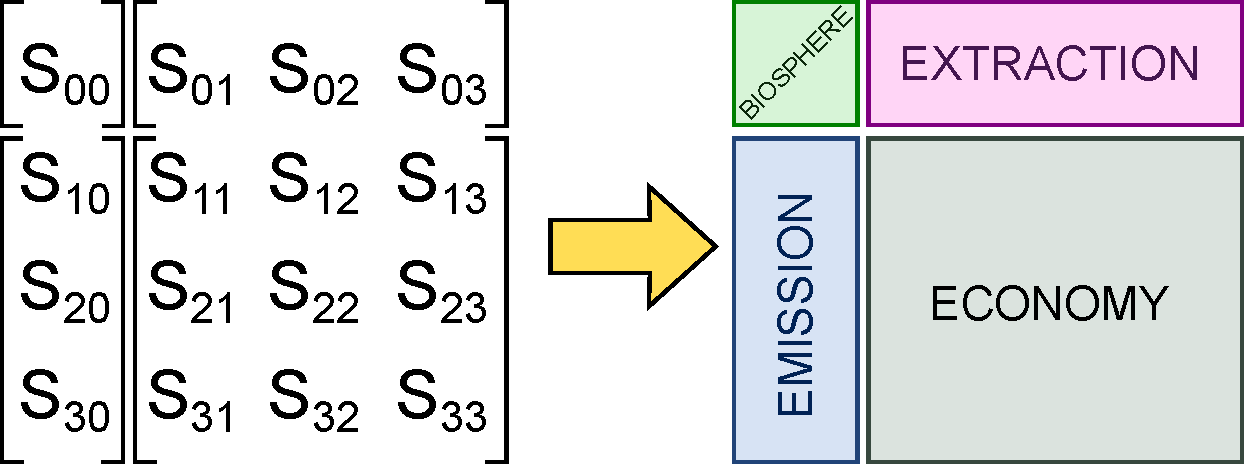
\includegraphics[width=0.8\linewidth]{Part_1/Chapter_Materials/images/Matrix.pdf}
\caption[The matrix of biosphere-economy flows]{The matrix of biosphere-economy flows. 
				Note that flow $\dot{S}_{00}$ is not included within our framework.}
\label{fig:C_mat_matrix}
\end{figure}

\begin{figure}[!ht]
\centering\
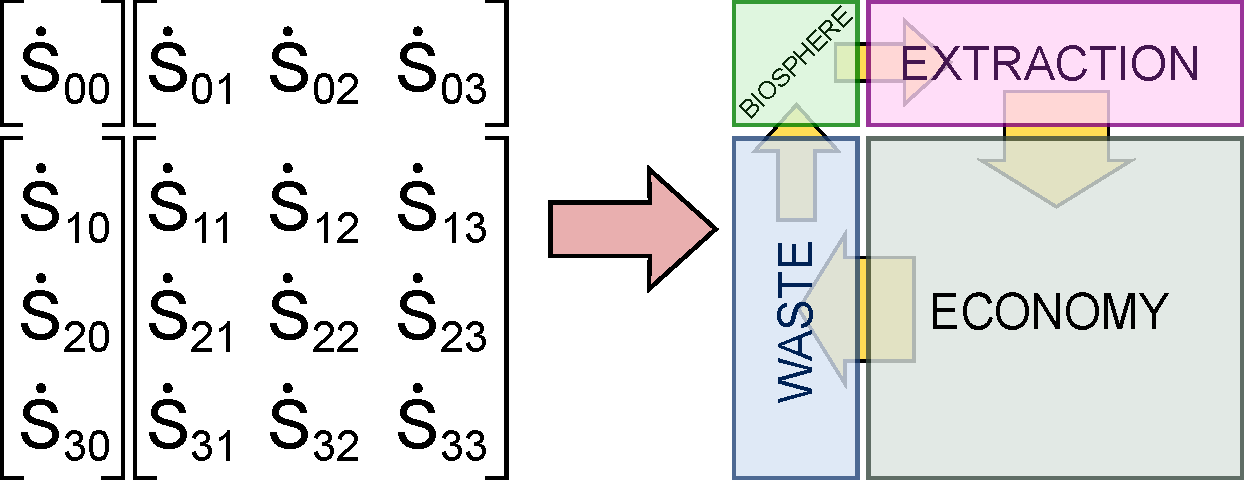
\includegraphics[width=0.8\linewidth]{Part_1/Chapter_Materials/images/Matrix_v2.pdf}
\caption[The matrix of biosphere-economy flows]{The matrix of biosphere-economy flows. 
				Note that flow $\dot{S}_{00}$ is not included within our framework.}
\label{fig:C_mat_matrix}
\end{figure}


%%%%%%%%%% Materials: Auto industry example %%%%%%%%%%
\section{Materials in the US auto industry}
\label{sec:materials_auto}
%%%%%%%%%%

Throughout the book, we shall be applying the methodology
that has been outlined through Examples~A-C to the
real-world case of the US auto industry.
The running example of the US auto industry demonstrates that our dynamic model 
can be tied into national accounts.
The US auto industry example shows where data are available 
(e.g., economic value, Chapter~\ref{chap:value}), 
where it is old (e.g., energy intensity, Chapter~\ref{chap:intensity}), 
and where it has never been available 
(e.g., accumulated embodied energy, Chapter~\ref{chap:embodied_energy}).  
The US auto industry is, therefore, 
illustrative of the challenges inherent 
in obtaining data that would feed the model.

The auto industry 
has been used previously
in the literature in both 
process-based~\cite{Berry:1973vo, Sullivan1995, Stodolsky1995, 
							Sullivan1998, McCleese2002, Sullivan2010, Hawkins2012}
and Input-Output~\cite{Bullard:1978vd, MacLean1998, MacLean2003}
analysis methods,
Furthermore, the industry
remains a large portion of many industrialized economies, 
is very resource intensive, 
has obvious links with energy because
its health is sensitive to disruptions in energy supplies, and
the industry also shows evidence of 
post-industrial decline (shrinking profit margins, etc.).

In Figure~\ref{fig:PERKS_materials_auto}
we see the flows of resources,
short-lived, and capital materials
into the auto industry.
Because the industry does not
extract resources directly from the biosphere,
the rate of flow of resources ($\dot{R}_{0j}$) 
from the biosphere to the auto industry 
has a zero value.
Each of the other flows represented in the diagram is,
in actuality,
a vector of hundreds (or even thousands!)
of elemental material flows,
each of which must be accounted 
(and balanced) separately.

There are a number of key material inputs into the
production of automobiles, directly as 
resources~($\dot{R}$) as well as short-lived 
materials~($\dot{S}$) and capital goods~($\dot{K}$)
outlined in Table~\ref{tab:materials_auto}. 
%**** MCD---split list into resources, short-lived and capital flows as table both inputs and outputs. 
% Maybe add annotation to Figure~\ref{fig:PERKS_materials_auto} ****
%**** MCD - Talk about the different materials:
%steel, glass, rubber, concrete, electricity, plastic
%finished product is automobile. 
%Emissions to air and water.
%Talk to financial (value) flows in Section~\ref{sec:value_auto} 
%as proxy for physical flows****
%**** This paragraph is kind-of unclear. Rewrite for clarity?---MKH ****
Data on the actual flow rates %**** What do you mean by ``rest of the flows?''
% Do you mean that mass-based, as opposed to dollar-based data are hard to find? ---MKH ****
at the industry level
is very hard to obtain.\footnote{The issue of 
lack of physical flow data is discussed in 
Section~\ref{sec:Data}.
}
In Europe,
economy-wide material flow accounts (EW-MFA)
have been produced by measurement of the physical flows
of materials into and out of economies of 
each of the member states.\cite{EUROSTAT2011} 
Work is ongoing to characterize the inter-sectoral
flows of these materials~\cite{ConAccount1998}
which can be analyzed by converting financial data 
(which is available, as discussed in 
Section~\ref{sec:value_auto}) into physical flow data
via knowledge of the entry points of materials into the economy,
i.e.\ via the extraction industries.

A number of studies have looked at 
the material and energy flows 
associated with specific or representative vehicle manufacturing 
\emph{processes}, rather than industry-level
activity.\cite{Sullivan1998, MacLean1998,Schweimer2000,
McCleese2002,MacLean2003, Burnham2006,Sullivan2010, Hawkins2012}
The US automobile industry is composed
of many such manufacturing processes.
According to the International Organization of 
Motor Vehicle Manufacturers~(OICA), 
2.7 million cars were produced in 2010\footnote{In 2006, 
prior to the Great Recession, 
the automobile industry purchased 
40 trillion kJ ($4.0 \times 10^{13}$ kJ) of total energy and 
produced 4.4 million cars.
} 
in the US.\cite{Motor-Vehicle-Manufacturers-OICA:2014aa}
In theory,
a representation of the industry-level flows
could be ``built up'' by assuming that the results from
these process-based analysis methods represent average
processes within the whole industry and 
scaling the material flows accordingly,
with appropriately wide uncertainty bounds.


%**** MCD---I'm not sure what else I can write here.
%% I could talk about process-based models? 
%Talk about other industries
%that may have better data.
%Signpost the issue of lack of data in Section~\ref{sec:Data}
%****

\begin{figure}[!ht]
\centering
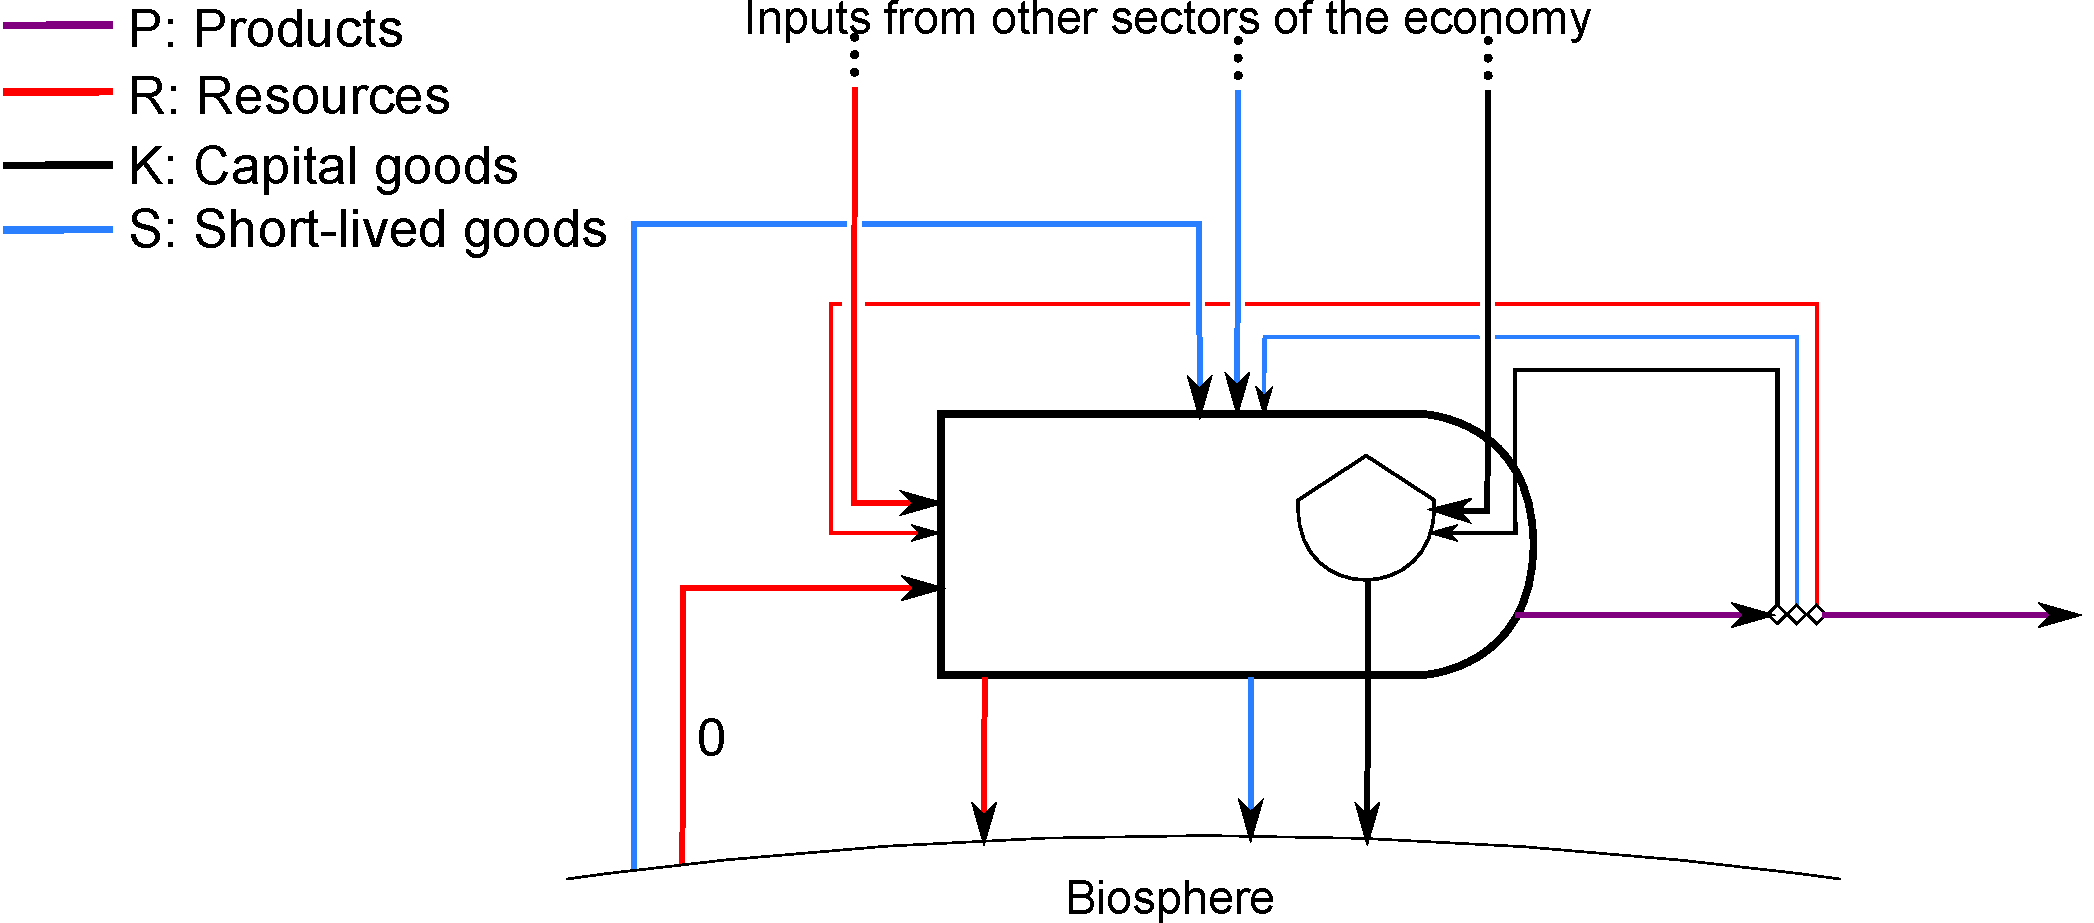
\includegraphics[width=\linewidth]{Part_1/Chapter_Materials/images/PERKS_basic_unit_materials_auto_ind.pdf}
\caption[Material flows for the US automobile industry]{Material 
flows for the US automobile industry using data from~\cite{Sullivan1998, 
MacLean1998,Schweimer2000, McCleese2002,MacLean2003, Burnham2006,
Sullivan2010, Hawkins2012}.}
\label{fig:PERKS_materials_auto}
\end{figure}

\begin{table}
\caption[List of material input and output flows for the 
US auto industry]{List of material input and output flows for 
the US auto industry (IOC:3361MV) 
as resources ($\dot{R}$),
short-lived materials ($\dot{S}$),
and capital goods ($\dot{K}$)
using data from~\cite{Sullivan1998, MacLean1998,Schweimer2000,
McCleese2002,MacLean2003, Burnham2006,Sullivan2010, Hawkins2012}.
This list is illustrative and by no means exhaustive.
%**** I thought there is very little COAL input to the auto industry. 
%Compare to Becky's table.---MKH ****
}
\begin{center}
 \begin{tabular}{p{4cm}p{1cm}p{5.2cm}}
\toprule 
\textbf{Material Flow}		 		& 								& \textbf{Materials} 									\\
\midrule
Resources from biosphere		& $\dot{R}_{0j}$		& none															\\[0.15cm]
Short-lived from biosphere		&	$\dot{S}_{0j}$	& oxygen, nitrogen, water							\\
\midrule
Resources from other sectors	& $\dot{R}_{ij}$		&	 cast iron (engine block);							\\
												&								&	 steel (chassis, panels);							\\
												&								&	 aluminum (body parts); 							\\		
												&								&	 copper (wiring);										\\	
												&								&	 zinc, chromium, carbon (alloying); 			\\
												&								&	 lead, nickel (battery cells);		 				\\
												&								&	 glass (windows, wind shield);					\\
												&								&	 rubber (tires);											\\
												&								&	 plastic (bodywork, interiors, seals)			\\
												&								&	 petroleum (paints, lubricants)					\\[0.15cm]
Short-lived from other sectors	& $\dot{S}_{ij}$		&	 energy (oil, natural gas, electricity)			\\
												&								&	 water (process)										\\
												&								&	 petroleum (solvents)								\\
												&								&	 plastic (packaging)									\\
												&								&	 paper (towels, packaging)						\\[0.15cm]
Capital from other sectors		& $\dot{K}_{ij}$		&	 steel (buildings, equipment)					\\
												&								&	 concrete (buildings)								\\
												&								&	 	glass (windows, screens)						\\
												&								&	 plastic (fixtures, fittings, equipment)		\\
												&								&	 	petroleum (paints, lubricants)				\\
\midrule
Product output							&	$\dot{P}_{j}$		&	auto parts and motor vehicles					\\[0.15cm]
\midrule
Resource self-consumption		&	$\dot{R}_{jj}$		&	auto parts												\\[0.15cm]
Short-lived self-consumption   &	$\dot{S}_{jj}$		&	none 														\\[0.15cm]
Capital self-consumption			&	$\dot{K}_{jj}$		&	motor vehicles											\\[0.15cm]
\midrule
Resources to biosphere			& $\dot{R}_{j0}$		&	trimmings and dust (metal, plastic, rubber)	\\[0.15cm]
Short-lived to biosphere			& $\dot{S}_{j0}$		&	air emissions (GHG, NO$_x$, SO$_x$)		\\
												&								& 	emissions to water									\\[0.15cm]
Capital to biosphere					& $\dot{K}_{j0}$	&	depreciated equipment								\\
												&								& 	depreciated buildings										\\
\bottomrule
\end{tabular}
\end{center}
\label{tab:materials_auto}
\end{table}


%%%%%%%%%% Materials: Summary %%%%%%%%%%
\section{Summary}
\label{sec:materials_summary}
%%%%%%%%%%

In this chapter we saw how we all use accounting in our everyday lives
to count not just physical things (people, apples) but also non-physical things
(money). We developed a rigorous procedure for accounting by defining the 
\emph{what}, \emph{when}, and \emph{where}: what are we counting,
when we begin and end counting,
and where is our system boundary (control volume) located. 
We saw that some things (e.g., apples) can be
created and destroyed, but other things (mass, energy)
are neither created nor destroyed.

We then applied this accounting procedure to materials 
flowing through an economy. 
We defined four different types of materials: \emph{resources},
\emph{short-lived goods}, and \emph{capital} which are used to make
\emph{products} and specified that only capital 
may accumulate within economic sectors.
We used these definitions in three examples,
building from a one-sector model of the economy
to a general framework for flows (and accumulation) 
of materials.
Finally, we applied the accounting framework to the 
real-world example of the US auto industry.
We categorized the types of materials used to produce
automobiles,
but found that industry-level data are difficult to obtain.

In the following two chapters of Part~\ref{part:matter},
we will apply our accounting framework 
to direct energy (Chapter~\ref{chap:direct_energy})
and embodied energy (Chapter~\ref{chap:embodied_energy}).

\bibliographystyle{unsrt}
\bibliography{../../Metabolic}


% Always give a unique label
% and use \ref{<label>} for cross-references
% and \cite{<label>} for bibliographic references
% use \sectionmark{}
% to alter or adjust the section heading in the running head
%% Instead of simply listing headings of different levels we recommend to let every heading be followed by at least a short passage of text. Furtheron please use the \LaTeX\ automatism for all your cross-references and citations.

%% Please note that the first line of text that follows a heading is not indented, whereas the first lines of all sequent paragraphs are.

%% Use the standard \verb|equation| environment to typeset your equations, e.g.
%
%% \begin{equation}
%% a \times b = c\;,
%% \end{equation}
%
%% however, for multiline equations we recommend to use the \verb|eqnarray|
%% environment\footnote{In physics texts please activate the class option \texttt{vecphys} to depict your vectors in \textbf{\itshape boldface-italic} type - as is customary for a wide range of physical jects.}.
%%\begin{eqnarray}
%%a \times b = c \nonumber\\
%% \vec{a} \cdot \vec{b}=\vec{c}
%% \label{eq:01}
%%\end{eqnarray}

%% \section{section Heading}
%% \label{sec:2}
%% Instead of simply listing headings of different levels we recommend to let every heading be followed by at least a short passage of text. Furtheron please use the \LaTeX\ automatism for all your cross-references\index{cross-references} and citations\index{citations} as has already been described in Sect.~\ref{sec:2}.

%% \begin{quotation}
%% Please do not use quotation marks when quoting texts! Simply use the \verb|quotation| environment -- it will automatically render Springer's preferred layout.
%% \end{quotation}


%% \section{section Heading}
%% Instead of simply listing headings of different levels we recommend to let every heading be followed by at least a short passage of text. Furtheron please use the \LaTeX\ automatism for all your cross-references and citations as has already been described in Sect.~\ref{sec:2}, see also Fig.~\ref{fig:1}\footnote{If you copy text passages, figures, or tables from other works, you must obtain \textit{permission} from the copyright holder (usually the original publisher). Please enclose the signed permission with the manucript. The sources\index{permission to print} must be acknowledged either in the captions, as footnotes or in a separate section of the book.}

%% Please note that the first line of text that follows a heading is not indented, whereas the first lines of all sequent paragraphs are.

% For figures use
%
%% \begin{figure}[b]
%% \sidecaption
% Use the relevant command for your figure-insertion program
% to insert the figure file.
% For example, with the option graphics use
%% \includegraphics[scale=.65]{figure}
%
% If not, use
%\picplace{5cm}{2cm} % Give the correct figure height and width in cm
%
%% \caption{If the width of the figure is less than 7.8 cm use the \texttt{sidecapion} command to flush the caption on the left side of the page. If the figure is positioned at the top of the page, align the sidecaption with the top of the figure -- to achieve this you simply need to use the optional argument \texttt{[t]} with the \texttt{sidecaption} command}
%% \label{fig:1}       % Give a unique label
%% \end{figure}


%% \paragraph{Paragraph Heading} %
%% Instead of simply listing headings of different levels we recommend to let every heading be followed by at least a short passage of text. Furtheron please use the \LaTeX\ automatism for all your cross-references and citations as has already been described in Sect.~\ref{sec:2}.

%% Please note that the first line of text that follows a heading is not indented, whereas the first lines of all sequent paragraphs are.

%% For typesetting numbered lists we recommend to use the \verb|enumerate| environment -- it will automatically render Springer's preferred layout.

%% \begin{enumerate}
%% \item{Livelihood and survival mobility are oftentimes coutcomes of uneven socioeconomic development.}
%% \begin{enumerate}
%% \item{Livelihood and survival mobility are oftentimes coutcomes of uneven socioeconomic development.}
%% \item{Livelihood and survival mobility are oftentimes coutcomes of uneven socioeconomic development.}
%% \end{enumerate}
%% \item{Livelihood and survival mobility are oftentimes coutcomes of uneven socioeconomic development.}
%% \end{enumerate}


%% \paragraph{paragraph Heading} In order to avoid simply listing headings of different levels we recommend to let every heading be followed by at least a short passage of text. Use the \LaTeX\ automatism for all your cross-references and citations as has already been described in Sect.~\ref{sec:2}, see also Fig.~\ref{fig:2}.

%% Please note that the first line of text that follows a heading is not indented, whereas the first lines of all sequent paragraphs are.

%% For unnumbered list we recommend to use the \verb|itemize| environment -- it will automatically render Springer's preferred layout.

%% \begin{itemize}
%% \item{Livelihood and survival mobility are oftentimes coutcomes of uneven socioeconomic development, cf. Table~\ref{tab:1}.}
%% \begin{itemize}
%% \item{Livelihood and survival mobility are oftentimes coutcomes of uneven socioeconomic development.}
%% \item{Livelihood and survival mobility are oftentimes coutcomes of uneven socioeconomic development.}
%% \end{itemize}
%% \item{Livelihood and survival mobility are oftentimes coutcomes of uneven socioeconomic development.}
%% \end{itemize}

%% \begin{figure}[t]
%% \sidecaption[t]
% Use the relevant command for your figure-insertion program
% to insert the figure file.
% For example, with the option graphics use
%% \includegraphics[scale=.65]{figure}
%
% If not, use
%\picplace{5cm}{2cm} % Give the correct figure height and width in cm
%
%% \caption{Please write your figure caption here}
%% \label{fig:2}       % Give a unique label
%% \end{figure}

%% \runinhead{Run-in Heading Boldface Version} Use the \LaTeX\ automatism for all your cross-references and citations as has already been described in Sect.~\ref{sec:2}.

%% \runinhead{Run-in Heading Italic Version} Use the \LaTeX\ automatism for all your cross-refer\-ences and citations as has already been described in Sect.~\ref{sec:2}\index{paragraph}.
% Use the \index{} command to code your index words
%
% For tables use
%
%% \begin{table}
%% \caption{Please write your table caption here}
%% \label{tab:1}       % Give a unique label
%
% For LaTeX tables use
%
%% \begin{tabular}{p{2cm}p{2.4cm}p{2cm}p{4.9cm}}
%% \hline\noalign{\smallskip}
%% Classes & class & Length & Action Mechanism  \\
%% \noalign{\smallskip}\svhline\noalign{\smallskip}
%% Translation & mRNA$^a$  & 22 (19--25) & Translation repression, mRNA cleavage\\
%% Translation & mRNA cleavage & 21 & mRNA cleavage\\
%% Translation & mRNA  & 21--22 & mRNA cleavage\\
%%Translation & mRNA  & 24--26 & Histone and DNA Modification\\
%%\noalign{\smallskip}\hline\noalign{\smallskip}
%%\end{tabular}
%%$^a$ Table foot note (with superscript)
%%\end{table}
%
%% \section{Section Heading}
%%\label{sec:3}
% Always give a unique label
% and use \ref{<label>} for cross-references
% and \cite{<label>} for bibliographic references
% use \sectionmark{}
% to alter or adjust the section heading in the running head
%% Instead of simply listing headings of different levels we recommend to let every heading be followed by at least a short passage of text. Furtheron please use the \LaTeX\ automatism for all your cross-references and citations as has already been described in Sect.~\ref{sec:2}.

%% Please note that the first line of text that follows a heading is not indented, whereas the first lines of all sequent paragraphs are.

%%If you want to list definitions or the like we recommend to use the Springer-enhanced \verb|description| environment -- it will automatically render Springer's preferred layout.

%%\begin{description}[Type 1]
%%\item[Type 1]{That addresses central themes pertainng to migration, health, and disease. In Sect.~\ref{sec:1}, Wilson discusses the role of human migration in infectious disease distributions and patterns.}
%%\item[Type 2]{That addresses central themes pertainng to migration, health, and disease. In Sect.~\ref{sec:2}, Wilson discusses the role of human migration in infectious disease distributions and patterns.}
%%\end{description}

%%\section{section Heading} %
%% In order to avoid simply listing headings of different levels we recommend to let every heading be followed by at least a short passage of text. Use the \LaTeX\ automatism for all your cross-references and citations citations as has already been described in Sect.~\ref{sec:2}.

%% Please note that the first line of text that follows a heading is not indented, whereas the first lines of all sequent paragraphs are.

%% \begin{svgraybox}
%% If you want to emphasize complete paragraphs of texts we recommend to use the newly defined Springer class option \verb|graybox| and the newly defined environment \verb|svgraybox|. This will produce a 15 percent screened box 'behind' your text.

%% If you want to emphasize complete paragraphs of texts we recommend to use the newly defined Springer class option and environment \verb|svgraybox|. This will produce a 15 percent screened box 'behind' your text.
%% \end{svgraybox}


%% \section{section Heading}
%%Instead of simply listing headings of different levels we recommend to let every heading be followed by at least a short passage of text. Furtheron please use the \LaTeX\ automatism for all your cross-references and citations as has already been described in Sect.~\ref{sec:2}.

%% Please note that the first line of text that follows a heading is not indented, whereas the first lines of all sequent paragraphs are.

%% \begin{theorem}
%% Theorem text goes here.
%% \end{theorem}
%
% or
%
%% \begin{definition}
%% Definition text goes here.
%% \end{definition}

%% \begin{proof}
%\smartqed
%% Proof text goes here.
%% \qed
%% \end{proof}

%%\paragraph{Paragraph Heading} %
%% Instead of simply listing headings of different levels we recommend to let every heading be followed by at least a short passage of text. Furtheron please use the \LaTeX\ automatism for all your cross-references and citations as has already been described in Sect.~\ref{sec:2}.

%% Note that the first line of text that follows a heading is not indented, whereas the first lines of all subsequent paragraphs are.
%
% For built-in environments use
%
%%\begin{theorem}
%%Theorem text goes here.
%%\end{theorem}
%
%%\begin{definition}
%%Definition text goes here.
%%\end{definition}
%
%%\begin{proof}
%%\smartqed
%% Proof text goes here.
%%\qed
%%\end{proof}
%
%% \begin{acknowledgement}
%% If you want to include acknowledgments of assistance and the like at the end of an individual chapter please use the \verb|acknowledgement| environment -- it will automatically render Springer's preferred layout.
%% \end{acknowledgement}
%
%% \section*{Appendix}
%% \addcontentsline{toc}{section}{Appendix}
%
%% When placed at the end of a chapter or contribution (as opposed to at the end of the book), the numbering of tables, figures, and equations in the appendix section continues on from that in the main text. Hence please \textit{do not} use the \verb|appendix| command when writing an appendix at the end of your chapter or contribution. If there is only one the appendix is designated ``Appendix'', or ``Appendix 1'', or ``Appendix 2'', etc. if there is more than one.

%% \begin{equation}
%% a \times b = c
%% \end{equation}
% Problems or Exercises should be sorted chapterwise
%% \section*{Problems}
%% \addcontentsline{toc}{section}{Problems}
%
% Use the following environment.
% Don't forget to label each problem;
% the label is needed for the solutions' environment
%% \begin{prob}
%% \label{prob1}
%% A given problem or Excercise is described here. The
%% problem is described here. The problem is described here.
%% \end{prob}

%% \begin{prob}
%% \label{prob2}
%% \textbf{Problem Heading}\\
%% (a) The first part of the problem is described here.\\
%% (b) The second part of the problem is described here.
%% \end{prob}


